% don't remove the folling lines, and edit the defintion of \main if needed
\documentclass[../report.tex]{subfiles}
\providecommand{\main}{..}
\IfEq{\jobname}{\currfilebase}{\AtEndDocument{\biblio}}{}
% until here

%\usepackage{multicol} % Doesnt work? :(

\begin{document}

\section{High Energy Probes}

\subsection{tth differential measurements}
\subsection{WH/ZH at high energy/luminosity}
\begin{center}
\bigskip\vspace{1cm}
{Shankha Banerjee$^{a}$,  Rick S. Gupta$^{a}$,  Christoph Englert$^{b}$ and Michael Spannowsky$^{a}$}
\centerline{$^a${\it Institute of Particle Physics Phenomenology, Durham University, Durham DH1 3LE, UK}}
\centerline{$^b${SUPA, School of Physics and Astronomy, University of Glasgow, Glasgow G12 8QQ, UK}}
\end{center}
\large{\bf Introduction and EFT analysis} \\ \\

\normalsize
%%%%%%%%%%%%%%%%%%%%%%%%%%%%%%%%%%


In this note we perform a collider study of the Higgs-strahlung process, $pp \to Z(\ell^+ \ell^-)h(b\bar 
b)$ in the Standard Model Effective Field Theory (SMEFT) framework. We will see that the leading high energy contribution to the $pp \to Zh$ process comes from the four 
contact interactions  $hZ_\mu \bar{u}_{L,R} \gamma^\mu u_{L,R}$ and $hZ_\mu \bar{d}_{L,R} \gamma^\mu 
d_{L,R}$ that appear in the dimension-6 Lagrangian. These are the same four EFT directions, the so called ``high 
energy primaries'' that control  high energy $Wh,~WW$ and $WZ$ production (see Ref.~\cite{Franceschini:2017xkh}). The (pseudo-)observables involved in these diboson processes (anomalous TGCs and $Z$-pole observables)  have already been constrained at LEP.  We show in this note that    because of the higher  energies accessible at the LHC one can obtain bounds on these observables that are at least an order of magnitude stronger than those obtained at LEP.


The vertices in the dimension 6 Lagrangian that contribute 
to the $ff \to Vh$ (where $V=W,Z$) process in unitary gauge are as follows, 
\begin{eqnarray}
&&\Delta {\cal L}_6\supset \sum_f {\delta g^Z_{f}} Z_\mu \bar{f} \gamma^\mu f +\delta g^W_{ud} (W^+_\mu \bar{u}_L \gamma^\mu d_L+h.c.)
+ {g^h_{VV}}\,  h \left[W^{+\, \mu} W^-_\mu+\frac{1}{2c_{\theta_W}^2}Z^\mu Z_\mu\right]\nonumber \\
&&+  \delta g^h_{ZZ}\, h \frac{Z^\mu Z_\mu}{2c_{\theta_W}^2} + \sum_f g^h_{Zf}\,\frac{h}{v}Z_\mu \bar{f} \gamma^\mu f+g^h_{Wud}\,\frac{h}{v}(W^+_\mu \bar{u}_L \gamma^\mu d_L+h.c.)
+{\kappa_{Z \gamma }}\frac{h}{v} A^{\mu\nu} Z_{\mu\nu} \nonumber \\ 
&&+\kappa_{WW}\,\frac{h}{v}
 W^{+\, \mu\nu}W^-_{\mu\nu}
+\kappa_{ZZ}\,\frac{h}{2v} Z^{\mu\nu}Z_{\mu\nu}\,.
\label{lagr}
\end{eqnarray}
Here we have used the Lagrangian presented in Ref.~\cite{Gupta:2014rxa, Pomarol:2014dya}, where $\alpha_{em}$, $m_Z$ and $m_W$   have been used as input parameters and any corrections 
to the SM vector boson propagators  have 
been traded in favor of the vertex corrections. After summing over all $V$-polarizations, the leading 
piece in the high energy cross-section deviation for $ff \to Vh$ , is proportional to the four  contact interactions:  $g^h_{Zf}$, with $f=u_L, u_R,d_L$ and $d_R$.\footnote{There exists a basis independent constraint at the dimension-6 level, $\sqrt{2}\;g^h_{Wud}= (g^h_{Zd_L}-g^h_{Zu_L})$. } Table~\ref{dirn}, shows the linear combinations of Wilson coefficients contributing to the four 
$g^h_{Zf}$ couplings in different EFT bases.  The aforementioned directions are shown in the BSM Primary basis of Ref.~\cite{Gupta:2014rxa}, 
where the Wilson coefficients are already constrained pseudo-observables. In this basis we see that these can be written in terms of already constrained LEP (pseudo)observables. 

Given the inability to control the polarization of the initial state partons in a hadron collider, 
the process, in reality, only probes two of the above four directions. Taking only the interference 
term, we find these directions to be
\begin{equation}
g^Z_{\textbf{u}}= g^h_{Zu_L}+\frac{g^Z_{u_R}}{g^Z_{u_L}} g^h_{Zu_R},\; 
g^Z_{\textbf{d}}= g^h_{Zd_L}+\frac{g^Z_{d_R}}{g^Z_{d_L}} g^h_{Zd_R}\,.
\end{equation}
 %where $g^Z_f$ is defined below \eq{amps}. 
 At a given energy, a linear combination of the up-type and down-type coupling 
 deviations, enters the interference term for the 
 $pp \to Zh$ process, $g^Z_{\textbf{p}}= g^Z_{\textbf{u}}+ \frac{{\cal L}_d(\hat{s})}{{\cal L}_u(\hat{s})}g^Z_{\textbf{d}},$
where ${\cal L}_{u,d}$ is the $u \bar{u}$, $d \bar{d}$ luminosity at a given partonic centre of mass 
energy. The luminosity ratio changes very little with energy: between 0.65 and 0.59 as 
$\sqrt{\hat{s}}$ is varied from 1 to  2 TeV. Thus, to a good approximation, $pp \to Zh$ probes 
the single direction, 
\begin{equation}
g^Z_{\textbf{p}}=g^h_{Zu_L} -0.76~g^h_{Zd_L}   - 0.45~g^h_{Zu_R} + 0.14~g^h_{Zd_R}  \,.
\label{compdir}
\end{equation}
%where we have substituted the values for $g^Z_f$ and evaluated the luminosities at the energy 
using ${\hat{s}}=(1.5~\text{TeV})^2$. Using Tab.~\ref{dirn}, one can now write this in terms of the LEP-constrained pseudo-observables,
\begin{eqnarray}
g^h_{Z\textbf{p}}&=&2~\delta g^h_{Zu_L} -1.52~\delta g^h_{Zd_L}   - 0.90~\delta g^h_{Zu_R} + 0.28~\delta g^h_{Zd_R}\nonumber\\
&&-0.14~\delta \kappa_\gamma   -0.89~\delta g^Z_1 \nonumber\\
g^h_{Z\textbf{p}}&=&-0.14~(\delta \kappa_\gamma-\hat{S}+Y) -0.89~\delta g^Z_1  -1.3~W
\label{diru}
\end{eqnarray}
where the first  and second lines apply respectively to the general and universal case (third and fourth row of Table~\ref{dirn}). 
 
%%%%%%%%%%%%%%%%%%%%%%%%%%%%%%%%%%%
\begin{table*}[!t]
\begin{center}
\small
\begin{tabular}{|c|c|}%\hline
\hline
&EFT directions probed by high energy $ff \to Vh$ production \\
\hline
\hline
 Warsaw Basis~\cite{Grzadkowski:2010es} & $- \frac{2 g}{c_{\theta_W}}\frac{v^2}{\Lambda^2}(|T_3^f|c^{1}_L-T_3^f c^{3}_L+(1/2-|T_3^f|)c_f)$\\
BSM Primaries~\cite{Gupta:2014rxa} &$   \frac{2 g}{c_{\theta_W}}Y_f t_{\theta_W}^2 \delta \kappa_\gamma+2 \delta g^Z_{f}- \frac{2 g}{c_{\theta_W}}(T^f_3 c_{\theta_W}^2 + Y_f s_{\theta_W}^2)\delta g_1^Z $\\
 SILH Lagrangian~\cite{Giudice:2007fh} &$  \frac{g}{c_{\theta_W}}\frac{m_W^2}{\Lambda^2}(2 |T_3^f|\hat{c}_W-2t_{\theta_W}^2 Y_f \hat{c}_B)$\\
 Universal observables &$ \frac{2 g}{c_{\theta_W}}Y_f t_{\theta_W}^2  (\delta \kappa_\gamma-\hat{S}+Y)- \frac{2 g}{c_{\theta_W}}(T^f_3 c_{\theta_W}^2 + Y_f s_{\theta_W}^2)\delta g_1^Z- \frac{2 g}{c_{\theta_W}}T^f_3 W$\\
 High Energy Primaries~\cite{Franceschini:2017xkh} &$ -\frac{2 m_W^2}{g c_{\theta_W} }(|T_3^f| a_q^{(1)}-T_3^f a_q^{(3)}+(1/2-|T_3^f|)a_f)$\\
\hline
 \end{tabular}
  \caption{ The linear combinations of Wilson coefficients contributing to the contact interaction couplings $g^h_{Zf}$where  $f=u_L, d_L, u_R, d_R$. the direction for a given $f$  can  be read off from this table by substituting the corresponding  value of the $SU(2)_L$ and $U(1)_Y$ quantum numbers  $T_3^f$ and $Y_f$. Here $\hat{c}_W=c_W+c_{HW}-c_{2W}$ and $\hat{c}_B= c_B+c_{HB}-c_{2B}$. For the nomenclature of the operators, their corresponding Wilson coefficients and observables see for eg. Ref.~\cite{Franceschini:2017xkh}.}
  \label{dirn}
\end{center}
\end{table*}

%%%%%%%%%%%%%%%%%%%%%%%%%%%%%%%%%%

To estimate  the cut-off for 
our EFT, note that the ${g}^h_{Vf}$ couplings arise from current-current operators that can be generated, for instance, 
by integrating out at tree-level a heavy $SU(2)_L$ triplet (singlet) vector $W'^a$ ($Z'$) that couples 
to SM fermion currents, $\bar{f} \sigma^a \gamma_\mu f$ ($\bar{f} \gamma_\mu f)$ with a coupling 
$g_f$ and to the Higgs current $i{H}^\dagger \sigma^a \lra{D}_\mu H$ ($i{H}^\dagger \lra{D}_\mu H$) 
with a coupling $g_H$. This gives ${g}^h_{Zf}\sim g_H g g_f v^2/\Lambda^2$,
where $\Lambda$ is the mass of the massive vector and thus the cut-off for our EFT description. A universal coupling to the SM fermions can arise  
via kinetic mixing of the heavy vector with the SM gauge bosons; this would give $g_f=g/2$ ($g_f=g' Y$), such that,
\begin{equation}
  \label{cutoff}
{g}^h_{Zu_L,d_L} \sim \frac{g_H g^2  v^2}{ 2\Lambda^2},\;
{g}^h_{Zu_R,d_R} \sim \frac{g_H g g' Y_{u_R,d_R} v^2}{\Lambda^2}.
\end{equation}
 For a given  set of couplings   $\{{g}^h_{Zu_L} ,{g}^h_{Zd_L} ,{g}^h_{Zu_R} ,{g}^h_{Zd_R} \}$, the cut-off is  evaluated using 
 Eq.~\ref{cutoff} with $g_H=1$ (note that this is somewhat larger than the value corresponding to the SM $hZZ$ coupling) and taking the smallest of the four values. \\ \\
 
                                                                                                                
% %%%%%%%%%%%%%%%%%%%%%%%%%%%%%%%%%%%                                                                                                              

\large{\bf Collider Analysis} \\ \\

\normalsize

For our collider analysis, we consider  $Z(\ell^+\ell^-)h$ production from a pair of quarks as well as from a 
pair of gluons.  For the decay of the Higgs boson,  we find that at an integrated luminosity of  300 fb$^{-1}$,  the diphoton mode is not feasible as it yields less than 5 events at high energies ($p_{T,Z}>150$ GeV). We thus focus on the decay $h\to b\bar b$ to obtain large statistics. The dominant backgrounds are then  
$Zb\bar{b}$ and the irreducible $Zh$ production in SM. Reducible contributions also arise from $Z+$ jets production (where we include $c$-quarks but do not require that they are explicitly tagged). We employ the BDRS 
approach~\cite{Butterworth:2008iy} and demand a fat jet with a cone radius of $R=1.2$. More details of the Monte-Carlo analysis, the QCD corrections, the detailed cut-based 
and multivariate analyses (MVA) can be found in Ref.~\cite{Banerjee:2018bio}. Finally, we find a cut-based (MVA) SM $Zh$ to $Zb\bar{b}$ ratio of $\sim 0.26 \; 
(0.50)$.

%%%%%%%%%%%%%%%%%%%%%%%%%%%%%%%%%%%%
\begin{figure}[!t]
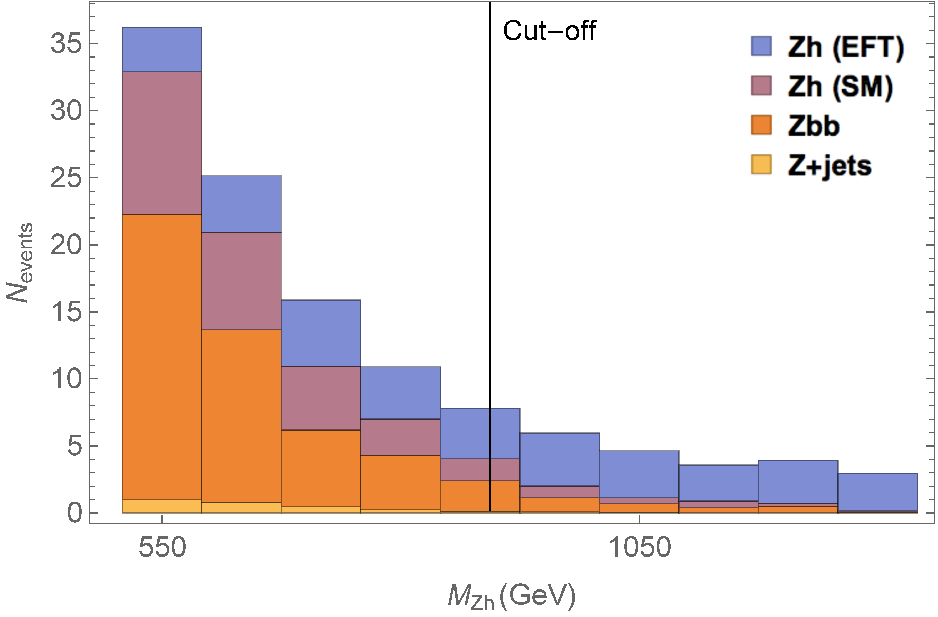
\includegraphics[width=0.45\textwidth]{\main/section4/bars}
\caption{The differential distribution of events at an integrated luminosity of 300 fb$^{-1}$ with respect to $M_{Zh}$ for the EFT signal as well as the different backgrounds. The EFT signal corresponds to the point $\{{g}^h_{Zu_L} ,{g}^h_{Zd_L} ,{g}^h_{Zu_R} ,{g}^h_{Zd_R} \}=\{-0.005, 0.0001 , -0.010, 0.005 \}$ which is allowed by  LEP bounds. The vertical line shows the cut-off evaluated using Eq.~\ref{cutoff}}
\label{bars}
\end{figure}
%%%%%%%%%%%%%%%%%%%%%%%%%%%%%%%%%%%%

To discriminate between the EFT signal and the irreducible SM $Zh(b\bar b)$ background we study  the 
growth of the EFT cross-section at high energies. This can be seen in Fig.~\ref{bars}  where we show the differential distribution with respect to $M_{Zh}$, the invariant mass of the leptons and the fat jet, for the EFT signal as well as for the different backgrounds. The EFT signal corresponds to a point that can be excluded in our analysis but is allowed by the LEP constraint.  To fully utilise the shape deviation of the EFT signal with respect to the background, 
we perform a binned log likelihood analysis assuming a 5$\%$ systematic error taking only events below the cut-off (evaluated as explained below Eq.~\ref{cutoff}). To obtain the   95$\%$ CL exclusion curve, we assume that 
the observed number of events would agree with the SM. \\ \\
%%%%%%%%%%%%%%%%%%%%%%%%%%%%%%%%%%
\large{\bf Discussion and Conclusions} \\ \\
%%%%%%%%%%%%%%%%%%%%%%%%%%%%%%%%%%
\normalsize
Taking into account only the SM-BSM interference term, we find the following per-mille level bounds for 300 (3000) fb$^{-1}$, 
\begin{equation}
g^h_{Z\textbf{p}} \in  \left[-0.004,0.004\right] \; (\left[-0.001,0.001\right])
\label{obo}
\end{equation}
The above bounds    translate to a lower bound on the scale of new physics given by 2.4 TeV (4.4 TeV) at 300 fb$^{-1}$ (3000 fb$^{-1}$) using Eq.~\ref{cutoff}.  To compare the above projections with existing LEP bounds, one can now extract bounds on the LEP observables contributing to $g^h_{Z\textbf{p}}$ in Eq.~\ref{diru} by turning them  on one by one. We show the results  in Tab.~\ref{lepb}. For the TGCs $\delta g^Z_1$ and $\delta \kappa_\gamma$, our projections are much stronger than the LEP bounds and  in the case of the $Z$-pole observables $\delta g^Z_f$, that parametrize the deviations of the $Z$ coupling to quarks, they are comparable. 

%%%%%%%%%%%%%%%%%%%%%%%%%%%%%%%%%%%%%%%%%%%%%%
\begin{figure}[!t]
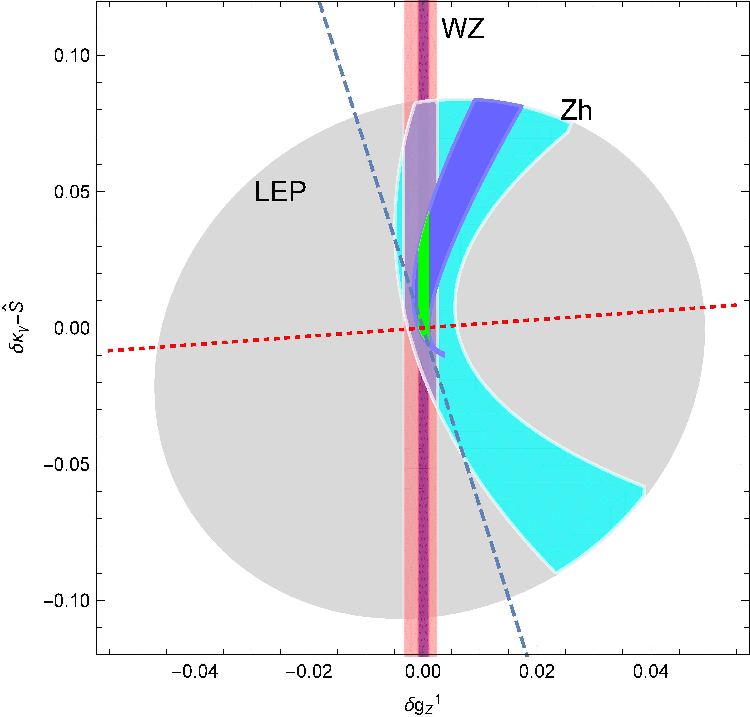
\includegraphics[width=0.45\textwidth]{\main/section4/300plot}
\caption{The light blue (dark blue) region above shows the projection for the allowed region with 300 fb$^{-1}$ (3 ab$^{-1}$) data from the 
$pp \to Zh$ process  in the $\delta \kappa_\gamma-\hat{S}$ vs $\delta g^Z_1$ plane for universal models. We show in grey the allowed region after LEP bounds (taking the TGC $\lambda_\gamma=0$, a conservative choice) are imposed.  In pink (dark pink)  we show the region that corresponds to the projection from the $WZ$ process  with 300 fb$^{-1}$ (3 ab$^{-1}$) data derived in Ref.~\cite{Franceschini:2017xkh} and the purple (green) region shows the region that survives from a combination of the $Zh$ and $WZ$ projections with 300 fb$^{-1}$ (3 ab$^{-1}$) data.}\label{bounds}
\end{figure} 
%%%%%%%%%%%%%%%%%%%%%%%%%%%%%%%%%%%%

For the universal case, we perform a more detailed analysis. The results are shown in the 
$\delta \kappa_\gamma-\hat{S}$ vs. $\delta g^Z_1$ plane  in Fig.~\ref{bounds} for the interesting class of models where $W=Y=0$~\cite{Franceschini:2017xkh}. The  
direction related to the $pp \to Zh$ interference term, \textit{i.e.}, $g^h_{Z\textbf{p}}=0$ (see Eq.~\ref{compdir} and the second line of Eq.~\ref{diru}) is shown by the dashed blue line, whereas the direction orthogonal to it is shown by the dotted red line.  Once the LEP II bounds~\cite{LEP2} from the $e^+e^- \to W^+W^-$ 
process are imposed, the allowed region that remains is shown by the grey shaded area. We show the results of this work  in blue (light (dark) blue for results at
300 (3000) fb$^{-1}$).  The shape of the allowed region arises due to the fact that the interference term vanishes along the dashed blue line and the squared term increases in magnitude as we move away from the origin. This curves the allowed region away from the dashed line as we move away from the origin.  The accidental cancellation of the interference term means that our bounds are susceptible to dimension-8 effects along this direction. On the other hand our bounds are more robust and not susceptible to such effects in the orthogonal direction shown by the red dotted line.

%%%%%%%%%%%%%%%%%%%%%%%%%%%%%%%%%%
\begin{table}[t]
\begin{center}

\begin{tabular}{c|c|c}%\hline
&Our Projection &LEP Bound\\\hline
$\delta g^Z_{u_L}$         & $\pm0.002~(\pm0.0007)$ & $-0.0026\pm 0.0016$\\
$\delta g^Z_{d_L}$         & $\pm0.003~(\pm0.001)$  & $0.0023\pm 0.001$\\
$\delta g^Z_{u_R}$         & $\pm0.005~(\pm0.001)$  & $-0.0036\pm 0.0035$\\
$\delta g^Z_{d_R}$         & $\pm0.016~(\pm0.005)$  & $0.0016\pm 0.0052$\\
$\delta g^Z_1$             & $\pm0.005~(\pm0.001)$  & $0.009^{+0.043}_{-0.042}$\\
$\delta \kappa_\gamma$     & $\pm0.032~(\pm0.009)$  & $0.016^{+0.085}_{-0.096}$\\
$\hat{S}$                  & $\pm0.032~(\pm0.009)$ & $0.0004 \pm 0.0007$\\
$W$                        & $\pm0.003~(\pm0.001)$  & $0.0000 \pm 0.0006$\\
$Y$                        & $\pm0.032~(\pm0.009)$  & $0.0003\pm 0.0006$
 \end{tabular}
  \caption{Comparison of the bounds obtained in this work with existing LEP bounds obtained by turning on the LEP observables in Eq.~\ref{diru} one by one and using Eq.~\ref{obo}. The LEP bounds on the $Z$ coupling to quarks has been obtained from Ref.~\cite{Falkowski:2014tna}, the bound on the TGCs from Ref.~\cite{LEP2}, the bound on $\hat{S}$ from Ref.~\cite{Baak:2012kk} and  finally the bounds on $W,Y$ have been obtained from Ref.~\cite{Barbieri:2004qk}. Except for the case of the bounds on $\delta g^Z_f$, all of the bounds in the last column were derived by turning on only the given parameter and putting all other parameters  to zero. The numbers outside (inside) brackets, 
  in the second column, denote our bounds with $\mathcal{L} = 300 \; (3000)$ fb$^{-1}$.  \label{lepb}}
\end{center}
\end{table}
%%%%%%%%%%%%%%%%%%%%%%%%%%%%%%%%%%

As $VV$ production constrains the same set of operators as the $Vh$ 
production in Fig.~\ref{bounds}, we also show the projected bound from the $WZ$ process at 300 
fb$^{-1}$ obtained in Ref.~\cite{Franceschini:2017xkh}. Only the 
purple region remains when both these bounds are combined  at 300 fb$^{-1}$. This shrinks further to the green region  at 3000 fb$^{-1}$. A drastic reduction in the allowed LEP region is   thus possible by considering the $pp \to Zh$ at high energies.

\subsection{ Electroweak Precision Tests  in High-Energy Diboson Processes} 
\begin{center}
\bigskip\vspace{1cm}
{Roberto Franceschini$^{a}$,  Giuliano Panico$^{b}$,  Alex Pomarol$^{b,c}$,\\
  Francesco Riva$^d$  and Andrea Wulzer$^{d,e,f}$}
\centerline{$^a${\it Dipartimento di Matematica e Fisica, Universit\`a di Roma Tre and INFN, 
%sezione di Roma Tre, 
00146~Rome}}
\centerline{$^b${\it \small IFAE and BIST, Universitat Aut\`onoma de Barcelona, 08193~Bellaterra,~Barcelona}}
\centerline{$^c${\it \small Dept.~de~F\'isica, Universitat Aut{\`o}noma de Barcelona, 08193~Bellaterra,~Barcelona}}
\centerline{$^d${\it\small Theoretical Physics Department, CERN, Geneva, Switzerland}}
\centerline{$^e${\it \small Institut de Th\'eorie des Ph\'enomenes Physiques, EPFL, Lausanne, Switzerland}}
\centerline{$^f${\it \small Dipartimento di Fisica e Astronomia, Universit\'a di Padova and INFN Padova, Italy}}
\end{center}

\noindent
{\bf High-Energy Primary Effects in Diboson Production}\\
Diboson production processes provide a very good sensitivity to a large set of new-physics effects and can be effectively used
to test interesting classes of BSM theories. In this section we classify the leading new-physics effects that can be tested
in these channels, showing that they can be encapsulated in four real ``high-energy primary'' (HEP) parameters~\cite{Franceschini:2017ab} .
We also assess the reach on these parameters at the HL-LHC and at future hadronic colliders, focusing in particular
on the fully leptonic $WZ$ channel that appears particularly promising.

We are interested in processes which fulfill two conditions. First, their amplitudes must receive BSM contributions that grow with $E^2$ at the leading order (i.e., $d=6$) in the EFT operator expansion. Second, the  SM amplitudes must be constant and sizable
at high energy, in such a way that, at the linear order in the EFT Wilson coefficient,  the $E^2$-growth of the BSM amplitudes
results into a $E^2$-growth of the differential cross-sections thanks to the SM-BSM interference. 
As explained in detail in Ref.~\cite{Franceschini:2017ab}, only $pp \to V_LV_L $ and $pp \to V_L h$ production
processes  enjoy quadratic energy growth at the interference level; we thus focus on these in the rest of the
section.\footnote{Notice however that promising strategies to circumvent the non-interference problem have been recently proposed \cite{Panico:2017frx,Azatov:2017kzw}, which allow for instance to ``resurrect'' interference effects in transverse vector bosons production.}
%\subsection{High-Energy Primary Effects}
The study of longitudinally-polarized dibosons production in the high-energy limit $E\gg m_{W}$ is greatly simplified
by using the Equivalence Theorem~\cite{Chanowitz:1985hj,Wulzer:2013mza}.
In this formalism, external longitudinally-polarized vector states are represented in Feynman diagrams as the corresponding
scalar Goldstone bosons, up to corrections of order $m_W/E$ from diagrams with gauge external lines.
%Furthermore, the $E\gg m_W$ limit can be safely taken in the internal line propagators and in the vertices, making that
%all the effects (masses and vertices) induced by the Higgs VEV manifestly produce order $m_W/E$ corrections.
In order to assess the leading energy behavior, it is sufficient to study the amplitude in the unbroken phase,
where the EW bosons are massless and the $G_{\rm{SM}}={\textrm{SU}}(2)_L\times{\textrm{U}}(1)_Y$ symmetry is exact.
Given that the Goldstone bosons live in the Higgs doublet $H$, together with the Higgs particle, $G_{\rm{SM}}$ implies
that the high-energy behavior of the former ones are connected with the latter. This is the reason why $V_LV_L$
and $V_Lh$ production processes, collectively denoted as $\Phi\Phi'$ in what follows, should be considered together.

Focusing our interest to the production of $\Phi\Phi'$ out of a quark $q'$ with helicity $\lambda'$ and an anti-quark ${\overline{q}}$ with helicity $\lambda$ we can restrict the form of the BSM amplitudes that interfere with SM one.
%As explained in detail in \cite{Franceschini:2017ab}  the dominance of J=1 SM amplitudes (up to corrections proportional to the light quark masses).
At order  $E^2/M^2$ in the EFT expansion the relevant BSM effects can be parametrized as corrections to the $J=1$ partial wave amplitudes~\cite{Franceschini:2017ab}, namely
\begin{equation}\label{amp0}
\delta{\mathcal{A}}\left(q^\prime_{\pm}{\overline{q}}_{\mp}\rightarrow\Phi\Phi'\right)= f^{\Phi\Phi'}_{q^\prime_{\pm}{\overline{q}}_{\mp}}(s)\sin\theta=  \frac{1}{4} A^{\Phi\Phi'}_{q^\prime_{\pm}{\overline{q}}_{\mp}}\, E^2 \sin\theta^*\,,
\end{equation}
where $\theta^*$ is the scattering angle in the $\Phi\Phi'$ center of mass, and $E=\sqrt{s}$ is the center of mass energy.

Eq.~(\ref{amp0}) shows that at the leading order in the SM EFT expansion each diboson process is sensitive at high energy to a single constant new-physics parameter $A^{\Phi\Phi'}_{q^\prime_{\pm}{\overline{q}}_{\mp}}$ for every combination of initial or final states. This can be taken real since its imaginary part does not interfere with the SM. In addition, the SM symmetry group, which is restored in the high-energy limit, as previously explained, implies  several relations among these parameters~\cite{Franceschini:2017ab}. %These relations can be found in Ref.~\cite{Franceschini:2017ab}, here we 
As a consequence, only $4$ HEP parameters are enough to parametrize the BSM effects we are interested in. This is very non-trivial from an EFT perspective, since a total of $6$ anomalous couplings coming from $d=6$ effective operators contribute to longitudinal diboson processes. These couplings can be identified as
${\delta g^Z_{uL}}$, ${\delta g^Z_{uR}}$, ${\delta g^Z_{dL}}$, ${\delta g^Z_{dR}}$, ${\delta g_1^Z}$ and ${\delta \kappa_{\gamma}}$ in the notation of Ref.~\cite{Gupta:2014rxa}.


The relations between the HEP parameters and the $4$ combinations of the low-energy primaries that produce growing-with-energy effects are reported in the third column of table~\ref{Wilsons}.

\begin{table}[t]
\begin{center}
\begin{tabular}{c|c|c}%\hline
Amplitude& High-energy primaries& Low-energy primaries  \\\hline
\rule[-1.4em]{0pt}{3.2em}$\bar u_L d_L\to W_LZ_L,W_Lh$ & $\sqrt{2}a_q^{(3)}$ & $ \displaystyle\sqrt{2}\frac{g^2}{m_W^2}\left[c_{\theta_W}({\delta g^Z_{uL}}-{\delta g^Z_{dL}})/g-c_{\theta_W}^2{\delta g_1^Z} \right]$ \\
\hline
\rule[-.6em]{0pt}{1.7em}$\bar u_L u_L\to W_LW_L$& \multirow{ 2}{*}{$a_q^{(1)}+a_q^{(3)}$}& \multirow{ 2}{*}{$\displaystyle-\frac{2g^2}{m_W^2}\left[Y_L t^2_{\theta_W}{\delta\kappa_\gamma}+T_Z^{u_L}{\delta g_1^Z}+c_{\theta_W}{\delta g^Z_{dL}}
%-\sqrt{2}{\delta g^W_L})
 /g\right]$}\\
\rule[-.55em]{0pt}{1.45em}$\bar d_L d_L\to Z_Lh$& &\\
\hline
\rule[-.6em]{0pt}{1.7em}$\bar d_L d_L\to W_LW_L$& \multirow{ 2}{*}{$a_q^{(1)}-a_q^{(3)}$}& \multirow{ 2}{*}{$\displaystyle-\frac{2g^2}{m_W^2}\left[Y_L t^2_{\theta_W}{\delta\kappa_\gamma}+T_Z^{d_L}{\delta g_1^Z}+c_{\theta_W}{\delta g^Z_{uL}}
%+\sqrt{2}{\delta g^W_L})
/g\right]$}\\
\rule[-.55em]{0pt}{1.45em}$\bar u_L u_L\to Z_Lh$& & \\
\hline
\rule[-1.2em]{0pt}{3.em}$\bar f_R f_R\to W_LW_L,Z_Lh$& $a_{f}$& $\displaystyle-\frac{2g^2}{m_W^2}\left[Y_{f_R} t^2_{\theta_W}{\delta\kappa_\gamma}+T_Z^{f_R}{\delta g_1^Z}+c_{\theta_W}{\delta g^Z_{fR}}/g\right]$
%\\\hline
 \end{tabular}
  \caption{Parameter combinations (in the high- and in the low-energy primary bases) that control $E^2$-enhanced effects in each polarized longitudinal diboson production process. Here, $T_Z^f=T_3^f-Q_fs^2_{\theta_W}$ and $Y_{L,f_R}$ is the hypercharge of the left-handed and right-handed quark (e.g., $Y_L=1/6$).}
\label{Wilsons}
\end{center}
\end{table}



The relations between the HEP and the Wilson coefficients in the SILH basis~\cite{Giudice:2007fh} are given by
\be
 a_q^{(3)}=\frac{g^2}{M^2}(c_W+c_{HW}-c_{2W})\ ,\ \  \ \
  a_q^{(1)}=\frac{g'^2}{3M^2}(c_B+c_{HB}-c_{2B})\,, \label{a2c}
\ee
and
\be
a_u=-2a_d=4 a_q^{(1)}\,.
\label{unifersal}
\ee
These relations can also be written using  the $\hat S$, $\hat T$, $W$ and $Y$ parameters (we follow the notation of Ref.~\cite{Barbieri:2004qk}) in addition to the two anomalous  triple gauge couplings (aTGC), $\delta g_1^Z$ and  $\delta \kappa_\gamma$. We have
\be
 a_q^{(3)}=-\frac{g^2}{m_W^2}\left(c^2_{\theta_W}\delta g_1^Z+W\right)\ ,\ \  \ \
  a_q^{(1)}=\frac{g'^2}{3m_W^2}\left(\hat S-\delta\kappa_\gamma+c^2_{\theta_W} \delta g_1^Z-Y\right)\,,
\label{heptosilh}  
\ee
which  can  be useful in order to  compare HEP analyses  from  LHC  with  other experiments, such as LEP. 



In the Warsaw basis \cite{Grzadkowski:2010es}, the HEP are transparently identified with contact interactions between quarks and scalars \footnote{These relations, as well as those in  \eq{a2c}, are obtained by computing the diboson helicity amplitudes in the presence of the EFT operators, and matching with the results of the low energy primaries. See Ref.~\cite{Franceschini:2017ab} for details.}
\be
a_u=4\frac{c_R^u}{M^2}\ ,\  \ a_d=4\frac{c_R^d}{M^2}\ ,\ \  a^{(1)}_q=4\frac{c^{(1)}_L}{M^2}\ ,\ \  a^{(3)}_q=4\frac{c^{(3)}_L}{M^2}\,.
\ee


%%%%%%%%%%%%%%%%%%%%%%%%%%%%%%%%%%%%%%%%%%%%%%%%%%%%%%%%%%%%%%%%%%%%%%%%%%%%%%%%%%%%%%%%%%%%%%%%%%%%%%%%%%%%%%%%%%%%%%%%%%%%%%%%%%%%%%%%%%
\vspace{1cm}
\noindent
{\bf LHC Primaries Sensitivity: The $\mathbf{WZ}$ Channel}\\
To illustrate the HE-LHC reach on the high-energy primaries we focus on $WZ$ production. This channel gives access to the
$a_q^{(3)}$ primary and has a very high sensitivity to new physics~\cite{Franceschini:2017ab}. We consider the fully leptonic final state
$$
pp\to W^{\pm}Z + {\rm{jets}}\to \ell\nu\ell^{\prime}\bar{\ell}^{\prime} + {\rm{jets}} \,, \;\;\; {\rm{with}}\;\;l,l'=e,\mu\,,
$$ 
which is likely to be measured with good accuracy and can benefit from a straightforward reconstruction of the final-state
leptons and a very low reducible background~\cite{Aad:2016ett}. At the experimental level
the situation might not be too much different from the neutral Drell-Yan process, in which a measurement with $2\%$
relative systematic uncertainty of the differential cross-section was performed, with run-$1$ LHC data,
up to TeV energies~\cite{Aad:2016zzw}.
A systematic uncertainty of $5\%$ might be considered as a realistic goal for the differential cross-section measurement in the leptonic $WZ$ channel. 

The main obstacle to obtain sensitivity to new physics is the potentially large contribution of the other polarizations, which for our purposes constitute a background, since they are insensitive to the new physics parameter $a_{q}^{(3)}$. In the $WZ$ channel these effects are automatically under control in the high-$p_T$ region and they can be further reduced by suitable selection criteria, as we will discuss later.

Due to the symmetry structure, the emission of transversely polarized $W$ and $Z$ bosons in the central rapidity region is disfavored~\cite{Franceschini:2017ab}. No suppression is instead expected for longitudinally polarized gauge bosons, therefore it is advantageous to concentrate our analysis on central scattering region, $|\cos \theta^*| \sim 0$, or, equivalently, at large $\ptv$ ($\ptv > 1\ {\rm TeV}$). We stress that other diboson processes, e.g. $pp \to WW$, do not enjoy this suppression of transverse vector boson emission, therefore are expected to be less sensitive probes of the high energy primaries. The interested reader can find estimates of the results achievable with the other diboson channels in Ref.~\cite{Franceschini:2017ab}.

\vspace{1cm}
\noindent
{\bf Analysis}\\
We now estimate the reach on $a_q^{(3)}$ based on a full NLO simulation of the $pp \to 3\ell\nu$ process. We report the analysis
of Ref.~\cite{Franceschini:2017ab} to which we refer for more details.
%We perform a matched calculation that uses matrix elements computed at NLO in QCD with {\sc{MadGraph5}} with FxFx-matched %\cite{Frederix:2012ly} parton shower supplied by Pythia8~\cite{Sjostrand:2014rr}, with NNPDF~2.3~NLO parton distributions. The %signal is computed through the operator $\op_{HW}$ implemented in the NLO version of the UFO model \texttt{EWdim6}.
We consider generation-level leptons momenta, but we include an overall detector efficiency for reconstructing the three leptons that we estimate around 50\%~\cite{ATLAS:2016iqc}. We furthermore apply standard acceptance cuts on the leptons (see Table~\ref{tab:cuts}).
%\be 
%p_{T,\ell}>30 \UGeV \ ,\quad |\eta_{\ell}|<2.4\,. \label{leptonscuts}
%\ee 
The same-flavor and opposite-charge lepton pair with invariant mass closer to the $Z$ boson mass is taken as the $Z$ candidate and the remaining lepton  is taken to be the decay product of the $W$ boson. The missing transverse energy vector of the event ($\cancel{\vec{E}}_T$ ) is estimated from the generation-level transverse neutrino momentum, to which we apply a Gaussian smearing with standard deviation
$ \sigma_{{\met}_{i}}^2 = (0.5)^2 \cdot \sum_f |p_i| \cdot {\rm{GeV}}\,$.
%This approach is similar to well-tested detector performance parameterizations used e.g.~in {\sc{Delphes}}~\cite{Ovyn:2009ys,de-Favereau:2013dk}.

\begin{table}
\centering
\begin{tabular}{c|c}
acceptance cuts &
$p_{T,\ell}>30 \UGeV \ ,\quad |\eta_{\ell}|<2.4$\\
\hline
\multirow{2}{*}{analysis cuts} &
$\deltapt/p_{T,V}<%[\deltapt/p_{T,V}]_{\rm{max}}=
0.5$\\
& $|\cos \thetastar| \leq %|\cos \thetastar|_{\rm{max}}=
0.5$
\end{tabular}
\caption{List of acceptance and analysis cuts.}\label{tab:cuts}
\end{table}

In order to highlight the production of longitudinally polarized vector bosons in the central rapidity region is useful to eliminate events with hard real radiation, which tend to be more abundant for our background of transverse polarized gauge bosons. To tame real radiation events in a controlled way we employ a selection on the transverse momentum of the $WZ$ system, denoted by $\deltapt=|{\vec{p}}_{T,W}+{\vec{p}}_{T,Z}|\,$.\footnote{Alternatively, a jet veto might be considered, which however could lead to lower accuracy because of the experimental and theoretical uncertainties in jets reconstruction.
%The $\deltapt$ variable is instead inclusive over the hadronic final state and it does not require jet reconstruction.
See also Ref.~\cite{Campanario:2014lza} for a different approach.} We require $\deltapt$ to be smaller than $50\%$ of the transverse momentum of the gauge bosons in the event, $p_{T,V} = \min(p_{T,W}, p_{T,Z})\,$. We also impose a cut on the scattering angle in the $WZ$ center of mass frame
$|\cos \thetastar| \leq  0.5\,$. The cuts are summarized in Table~\ref{tab:cuts}.



The kinematical variables described so far allow us to determine $p_{T,Z}$ and $p_{T,W}$, and in turn $p_{T,V}$ and $p_{T,VV}$, used to construct the binned distribution and for the selection cuts. In order to extract $|\cos \thetastar|$ the neutrino rapidity is reconstructed by the standard technique of imposing the invariant mass of the neutrino plus lepton system to be as close as possible to the physical $W$ boson mass.
A twofold ambiguity in the reconstruction is resolved by imposing the $|\cos \thetastar|$ cut on both solutions, i.e.~by retaining for the analysis only events such that both the possible neutrino configurations satisfy the selection criteria.

We study the $3$ collider energy options that correspond to the LHC ($14$~TeV), to the High-Energy LHC (HE-LHC, $27$~TeV) and to the FCC-hh ($100$~TeV). In each case we consider suitably designed $p_{T,V}$ bins, namely 
\begin{eqnarray}\label{finalbins}
{\textrm{LHC\hspace{-10pt}}}&{\textrm{:}}& p_{T,V}\in\{100,150,220,300,500,750,1200 \}\,,\\
{\textrm{HE-LHC\hspace{-10pt}}}&{\textrm{:}}& p_{T,V}\in\{150,220,300,500,750,1200, 1800 \}\,,\nonumber\\
{\textrm{FCC\hspace{-10pt}}}&{\textrm{:}}& p_{T,V}\in\{220,300,500,750,1200, 1800, 2400 \}\,.\nonumber
\end{eqnarray}
The binning is chosen such as to cover the kinematical regime that is accessible at each collider and it is taken as fine as possible in order to maximize the BSM sensitivity. On the other hand, a minimum bins size $\Delta p_{T,V}/ p_{T,V}\gtrsim30\%$ is required in order to avoid a degradation of the accuracy due to the $p_{T,V}$ resolution.



The predicted cross-sections are used to construct the $\chi^2$, under the assumption that observations  agree with the SM, and are eventually used to derive $95\%$~CL bounds on $a_q^{(3)}$. The uncertainties in each bin are the sum in quadrature of the statistical error, obtained from the SM expected events yield, and of a systematical component (uncorrelated across bins) which we take as a fixed fraction ($\delta_{\textrm{syst}}$) of the SM expectations. With this procedure we obtain, for different collider energies and luminosities and for $\delta_{\textrm{syst}}=5\%$
\bea
%{\textrm{LHC, }} 300\,{\textrm{fb}}^{-1}\hspace{-10pt} & {\textrm{:}} & a^{(3)}_q  \in  [-1.4, 0.9] \,10^{-1}\,\UTeV^{-2}\nonumber\\
{\textrm{HL-LHC, }} 3\,{\textrm{ab}}^{-1}\hspace{-10pt} & {\textrm{:}} & a^{(3)}_q  \in  [-4.9, 3.9] \,10^{-2}\,\UTeV^{-2}\nonumber\\
{\textrm{HE-LHC, }} 10\,{\textrm{ab}}^{-1}\hspace{-10pt} & {\textrm{:}} & a^{(3)}_q  \in  [-1.6, 1.3] \,10^{-2}\,\UTeV^{-2}\nonumber\\
{\textrm{FCC-hh, }} 20\,{\textrm{ab}}^{-1}\hspace{-10pt} & {\textrm{:}} & a^{(3)}_q  \in  [-7.3, 5.7] \,10^{-3}\,\UTeV^{-2}
\label{boundsf}
 \eea 
We see that the HE-LHC will improve the HL-LHC reach by a factor of $3$, while a gain of nearly one order of magnitude would be possible with the FCC-hh collider. The FCC-hh reach is comparable with the one of CLIC, as extracted from the analysis in Ref.~\cite{Ellis:2017kfi}.
 
%Notice that the choice $\delta_{\textrm{syst}}=5\%$ is not based on a careful assessment of the experimental systematical uncertainties and of the theory errors on the SM predictions. At the experimental level, we argued that $\delta_{\textrm{syst}}=5\%$ could be a reasonable target, based on analogies with other purely leptonic final states. For what concerns theory, parton luminosity uncertainties are well below $5\%$ in the energy range of interest and that the scale variations in the NLO calculation are of order $5\%$. Scale variations were estimated using MCFM~8.0~\cite{Boughezal:2016ek,Campbell:2011fp} by varying renormalization and factorization scale as $\mu_{R}=\mu_{F}=2^{\pm 1} (m_{W}+m_{Z})$. We will discuss later in this section how a larger or a smaller value of $\delta_{\textrm{syst}}$ would affect the reach.
 
The results of \eq{boundsf}  rely on BSM cross-section predictions obtained by integrating up to very high center of mass energies, formally up to the collider threshold. Therefore these limits assume that the description of the underlying BSM model offered by the EFT is trustable in the whole relevant kinematical regime, i.e.~that the cutoff $M$ of the BSM EFT is high enough. We quantify how large $M$ concretely needs to be for our results to hold by studying~\cite{Racco:2015dxa,Pobbe:2017wrj,Biekoetter:2014jwa} how the limit deteriorates if only events with low $WZ$ invariant mass, $m_{\textsc{wz}}<m_{\textsc{wz}}^{\rm{max}}$ are employed. This obviously ensures that the limit is consistently set within the range of validity of the EFT provided the EFT cutoff $M$ is below $m_{\textsc{wz}}^{\rm{max}}$. The results are reported in figure~\ref{fig:bounds_future}. Since the $95\%$~CL interval is nearly symmetric around the origin only the upper limit is reported in the figure for shortness.

\begin{figure}[t]
\centering
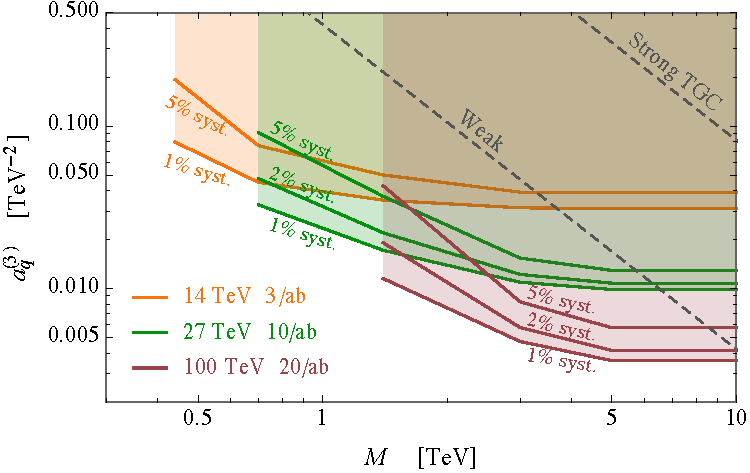
\includegraphics[width=0.7\textwidth]{\main/section4/MoneyPlotCombined}
\caption{Expected $95\%$ CL bounds from fully leptonic $WZ$ on the high-energy primary parameter $a^{(3)}_q$ as a function of the new physics scale $M$. The plots reports the results for the HL-LHC (orange lines), HE-LHC (green lines) and FCC-hh (brown lines) for different
values of the systematic uncertainties.} 
\label{fig:bounds_future}
\end{figure}

Several conclusions can be drawn from figure~\ref{fig:bounds_future}. First of all we see that the reach saturates for $m_{\textsc{wz}}^{\rm{max}}$ below around $1.5$~TeV at the HL-LHC if the systematic uncertainties are low, meaning that the limits obtained without $m_{\textsc{wz}}$ cut apply to theories with cutoff $M$ above that threshold.  The threshold grows to around $3$ and $4$~TeV at the HE-LHC and at the FCC-hh, respectively. The figures show that $\delta_{\textrm{syst}}=5\%$ is sufficient to probe ``Weak'' theories in all cases, but it also shows that the impact of larger or smaller uncertainties on the reach can be significant. Systematic errors at the $\delta_{\textrm{syst}}=5\%$ level already make an appreciable difference with respect to $\delta_{\textrm{syst}}=1\%$. This is due to the fact that the low-$p_{T,V}$ bins have small statistical error and the reach in those bins benefits from lower systematics. The effect is even more pronounced at the HE-LHC and at the FCC-hh, where even with $\delta_{\textrm{syst}}=2\%$ the reach deteriorates significantly with respect the ideal case $\delta_{\textrm{syst}}=1\%$. The fact that more accurate measurements would improve the reach of future colliders is an element that should be taken into account in the design of the corresponding detectors.

\subsection{Novel measurements of anomalous triple gauge couplings for the HE and HL-LHC} 
\begin{center}
\bigskip\vspace{1cm}{A. Azatov, D. Barducci, J. Elias-Mir\'o and Elena Venturini}
\\[7mm]
 {\it \small
SISSA and INFN sezione di Trieste, Via Bonomea 265; I-34137 Trieste, Italy\\
 }
\end{center}

\subsubsection{Introduction}
\label{intro}


In this work we are interested in the measurement of the Standard Model (SM) Triple Gauge Couplings (TGCs). This is a classic test of the SM and a possible measurement of deviations from its expectations would signify an invaluable piece of information for the theory beyond the SM. A consistent way to parametrize such possible deviations is through the SM Effective Field Theory (EFT) approach.
We are going to consider the SM EFT as defined in \cite{Azatov:2017kzw}, in particular we are going to focus on the measurement of the EFT operator 
\be
\mathcal{O}_{3W}=\frac{g}{3!}\epsilon^{abc} W^{a,\mu\nu}W_{\nu\rho}^b W_{\mu}^{c,\rho} \, , 
\ee
  which is associated to the the anomalous triple gauge coupling (aTGC) $\lambda_z$.





A precise determination of the TGC stems from the measurement of  the $2\to 2$  cross section $\sigma ( q\bar q \rightarrow VV )$~\cite{Sirunyan:2017bey,Aad:2016ett}. Naive dimensional analysis and standard EFT reasoning predicts that the energy scaling of such cross-section is given by
\bea
\label{eq:sigtt}
\begin{split}
\sigma(q\bar q \to V V)\sim \frac{g_{\text{SM}}^4}{E^2}\bigg[ 
 1 & +\overbrace{c_i\frac{E^2}{\Lambda^2}}^\text{BSM$_6\times\,$SM}
       +\overbrace{c_i^2 \frac{E^4}{\Lambda^4}}^\text{BSM$_6$$^2$}+ \dots \bigg]\, , 
\end{split} \label{genxsec}
\eea
where the first factor $g_\text{SM}^4/E^2$ accounts for the energy flux of the initial quarks, $c_i$ are the  relevant Wilson coefficients, and we have omitted numerical factors.
In (\ref{genxsec}) we have explicitly indicated dimension six squared  ($\text{BSM$_6$$^2$}$) and SM-dimension six interference terms ($\text{BSM$_6\times\,$SM}$).\footnote{Note that operators of dimension 7 necessarily violate either baryon or lepton number. We assume the scale of such symmetry violation to be very large and therefore irrelevant for diboson physics at the LHC.}  The ellipses in (\ref{genxsec}) are due to corrections from operators of dimension $\geq 8$, which we will neglect. The leading  such term is an interference term of the type $\text{BSM$_8\times\,$SM}$ and it is of order $O(E^4/\Lambda^4)$.

A closer inspection however reveals that the  $2\to 2$ diboson production through the dimension six operator $\mathcal{O}_{3W}$  has an interference piece with a suppressed energy scaling. 
Indeed, the energy scaling of such process is  
\begin{equation}
\sigma ( q\bar q \rightarrow VV ) \sim \frac{g_\text{SM}^4}{E^2}\bigg[  1 +  C_{3W}\frac{m_V^2}{\Lambda^2}  +C_{3W}^2 \frac{E^4}{\Lambda^4}  + O(E^4/\Lambda^4) \bigg]. \label{sup}
\end{equation} 
This is a consequence of the  helicity selection rules, see    
\cite{Dixon:1993xd,Azatov:2016sqh,Azatov:2017kzw,Panico:2017frx}.
The suppressed energy scaling can be problematic for the correct EFT  
interpretation of the $\sigma(q\bar q \to V V)$ measurement. 
Namely, in view of (\ref{sup}), the sensitivity on $C_{3W}$ is largely 
dominated by the quadratic piece $\text{BSM}_6^2$, which is 
$O(E^4/\Lambda^4)$. 
 Furthermore, in this case, the measurements become insensitive to the sign of the Wilson coefficient.
The main objective of the present work is to 
improve the sensitivity to the linear piece $\text{BSM$_6\times\,$SM}$.
We will present two classes of solutions to achieve this goal. Firstly, in section \ref{angs} we  will show that the differential angular cross-section 
 of the process $q\bar q \rightarrow VV\rightarrow 4\psi$ has a large sensitivity on $\text{BSM$_6\times\,$SM}$ compared to the inclusive cross-section.   Secondly, in section \ref{jetsol} we will show that accounting for extra radiation $q\bar q \rightarrow VV+j$ also results in an improved sensitivity on the leading piece $\text{BSM$_6\times\,$SM}$.
These measurements are specially interesting in a HL/HE phase of the LHC, for which we show the prospects in  section~\ref{res}.

\subsubsection{Solutions}


\begin{figure}[t]
\begin{center}
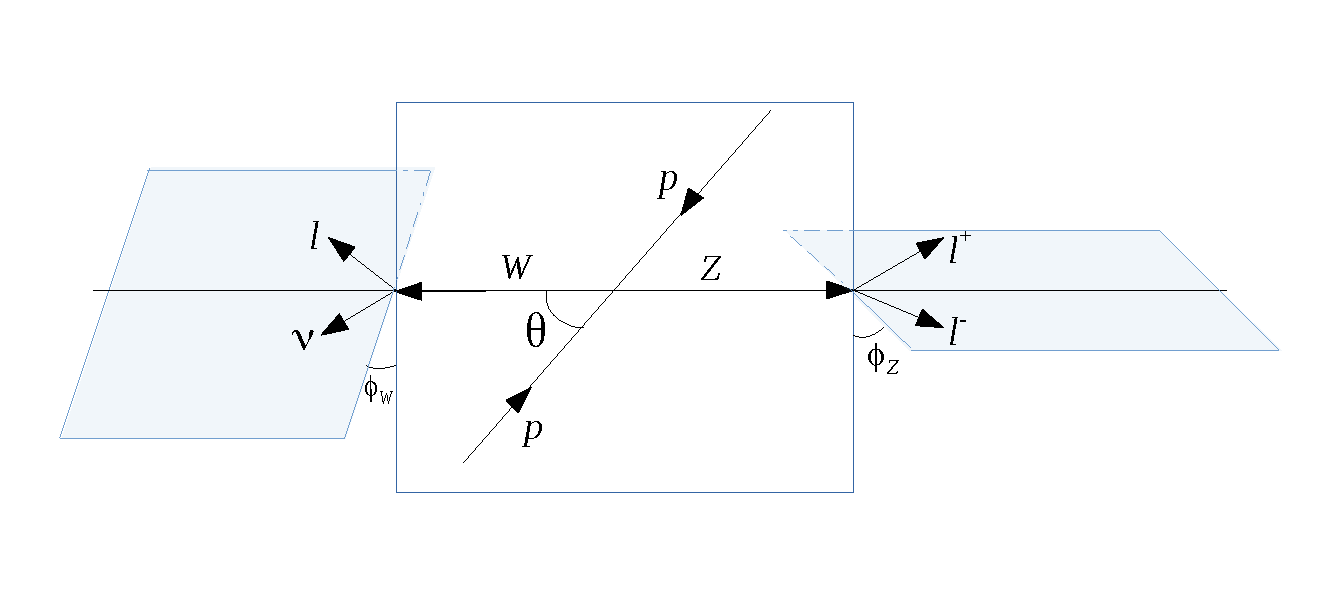
\includegraphics[scale=0.4]{\main/section4/angles}
\end{center}
\vspace{-.3cm}
\caption{Angles for $2\to 4$ scattering. \label{fig:ang}}
\end{figure}

Next we will present two ways to  improve the sensitivity to the aTGC $\lambda_z$ by restoring the energy growth
$g_\text{SM}^4/E^2\left[1+c_i E^2/\Lambda^2+  \dots\right]$ of the interference piece $\text{BSM$_6\times\,$SM}$ of the  $\mathcal{O}_{3W}$ operator.

\subsubsection*{Interference resurrection via angular distributions}
\label{angs}

The first way of enhancing the interference term is by noting that in a collider experiment instead of the  $2\to 2$ process we actually measure a $2\to 4$ scattering, i.e. vector bosons decay into fermions $q\bar q\to V_1V_2\to 4 \psi$.  

Let us start by considering  the differential cross section for the production of the polarized particles $W_{T+} Z_T \rightarrow W_{T+}  l_+ \bar l_-$\footnote{ We ignore the  longitudinal Z polarization which is subdominant at the LHC \cite{Baur:1994ia}.}
\be
\frac{d\sigma(q\bar q \rightarrow W_{T_+} l_- \bar l_+)}{d\text{LIPS} } =
 \frac{1}{2 s}  \frac{ \left|\sum_i  
(  {\cal M}^\text{SM}_{q\bar q \rightarrow W_{T_+}Z_{i}}+
 {\cal M}^\text{BSM}_{q\bar q \rightarrow W_{T_+}Z_{i}}
)
  {\cal M}_{Z_{i}\to  l_- \bar l_+}   \right|^2}{(k_Z^2-m_Z^2)^2+m_Z^2\Gamma_Z^2} 
\,  , \label{xsecan}
\ee
where   sum runs over intermediate Z polarizations and $d\text{LIPS}\equiv (2\pi)^4\delta^4(\sum p_i -p_f) \prod_i {d^3 p_i}/\left(2 E_i(2\pi)^3\right)$ is the Lorentz Invariant differential 
Phase Space.  
%
Then in the narrow width approximation the leading contribution to the interference, i.e. the cross term $\text{SM}\times\text{BSM}_6$ in \ref{xsecan},   is given by
$
d\sigma_\text{int}(q\bar q \rightarrow W_{T_+} l_- \bar l_+)/ d\phi_Z \propto E^2/\Lambda^2 \cos(2\phi_Z) 
$, 
where  $\phi_Z$  is the azimuthal angle between the plane defined by the decaying leptons and the plane defined by the collision and WZ momenta, see Fig.~\ref{fig:ang}.  Note that $d\sigma_\text{int}(q\bar q \rightarrow W_{T_+} l_- \bar l_+)/ d\phi_Z $ has the energy growth expected from naive dimensional analysis, see  Eq.~\ref{genxsec}.
An analogous derivation goes through if we also consider the decay of the W gauge boson. The differential interference term   for the process $q\bar q\to WZ\to 4 \psi$ is  unsuppressed and modulated as
\bea
 \frac{d\sigma_\text{int}(q\bar q \rightarrow W Z\rightarrow  4\psi)}{d\phi_Z\, d\phi_W}  \propto \frac{E^2}{\Lambda^2}\left( \cos(2\phi_Z)+\cos(2\phi_W)\right) , \label{simp}
\eea
where $\phi_{W,Z}$ are the corresponding azimuthal angles. 
Integrating  \ref{simp} over the fermion phase space the   interference term vanishes as expected from the discussion in section~\ref{intro}. 
Since the dependence on the two azimuthal angles is additive, integrating  over $\phi_W$ leads to a differential cross-section that is modulated by $\cos(2\phi_Z)$ and that features $E^2/\Lambda^2$ energy growth. 
We will use the result in Eq.~\ref{simp}  to prove the aTGC $\lambda_Z$, with an increased  overall sensitivity  to both the magnitude and sign of the Wilson coefficient.


 
\subsubsection*{Angle ambiguities \cite{Panico:2017frx}} 
 
 Let us make a few remarks on the experimental measurement  of $\phi_{Z,W}$ in Eq.~\ref{simp}.
 The angle $\phi_Z$  can be determined up to an ambiguity  $\phi_Z\leftrightarrow \phi_Z \pm \pi$,
 since experimentally we can only measure the charges but not the helicities of the  leptons from $Z$  decay.
 The reconstruction of the $W$  azimuthal  angle $\phi_W$ in the $l\nu$ final state  suffers from an ambiguity  $\phi_W \leftrightarrow \pi-\phi_W$ due to the twofold ambiguity in the determination of the neutrino momentum.
Interestingly, none of these ambiguities  affects  Eq.~\ref{simp}.

\subsubsection*{Interference resurrection via jet emission}
 \label{jetsol}
 
A second way to resurrect the expected energy growth of the 
interference term is based on the observation that the helicity 
selection rule holds only at tree-level \cite{Azatov:2017kzw}. 
So the next-to-leading-order (NLO) effects will necessarily lead to the 
enhancement of the interference.
Virtual effects are expected to be suppressed by a factor ${\cal{O}}( 
\alpha_s/4\pi)$ with respect to the contributions coming from 
azimuthal modulation discussed in the previous section.
Alternatively we will consider processes with an extra hard jet emission, which will improve on the  signal over the  background ratio. 
 In this case,  since   we are dealing with the hard
  $2\to 3$ process,
 the same polarization configuration $q\bar{q}\to V_{\pm}V_{\pm}g_{\mp}$ is allowed both in SM and in the BSM five point amplitude with the $\mathcal{O}_{3W}$ insertion. Therefore the interference is not suppressed and the leading quadratic energy scaling is restored by requiring an extra (hard) QCD radiation.


\subsubsection{Results}
\label{res}

\subsubsection*{HL-LHC}

In order to test the sensitivity of the High-Luminosity (HL) phase of the LHC on the $\mathcal{O}_{3W}$ with the proposed solution to the non-interference behaviour we proceed in the following way. We generate with {\tt MadGraph5 aMC@NLO}~\cite{Alwall:2014hca} parton level events for $pp \to W^{\pm} Z $ decaying into a four leptons (electron and muon) final state together with events for the same process where we allow for a jet emission in the initial state. We perform two different analyses (see~\cite{Azatov:2017kzw} for more details): an inclusive one where we restrict to events up to $p_T^j<100\;$ GeV and do not bin on the $\phi_Z$ variable and an exclusive one where we bin both on the jet transverse momentum and on $\phi_Z$, where for the latter we define two bins with the threshold $|\cos(\phi_Z)|=1/\sqrt{2}$. All together the results for the bound on the $C_{3W}$ Wilson coefficient are reported in Fig.~\ref{fig:LHC13} as a function of the maximum transverse mass of the $WZ$ system, which allows to have an estimate of the validity of the EFT computation, see again~\cite{Azatov:2017kzw} for a detailed discussion~\footnote{These results are obtained by keeping both the linear and the quadratic terms in the cross section determination.}.

One might wonder if a simulation beyond the parton level accuracy might spoil these results. To this end we have performed a more detailed simulation by showering the events through {\tt PYTHIA 8}~\cite{Alwall:2014hca} and simulating the detector response via {\tt Delphes 3}~\cite{deFavereau:2013fsa}. By analysing the density of events in the two azimuthal bins we found that with respect to the parton level case the relative difference is of at most a few \%, thus making our parton level analysis solid, see ref.~\cite{ade}.


  
  \begin{figure}[h!]
\begin{center}
 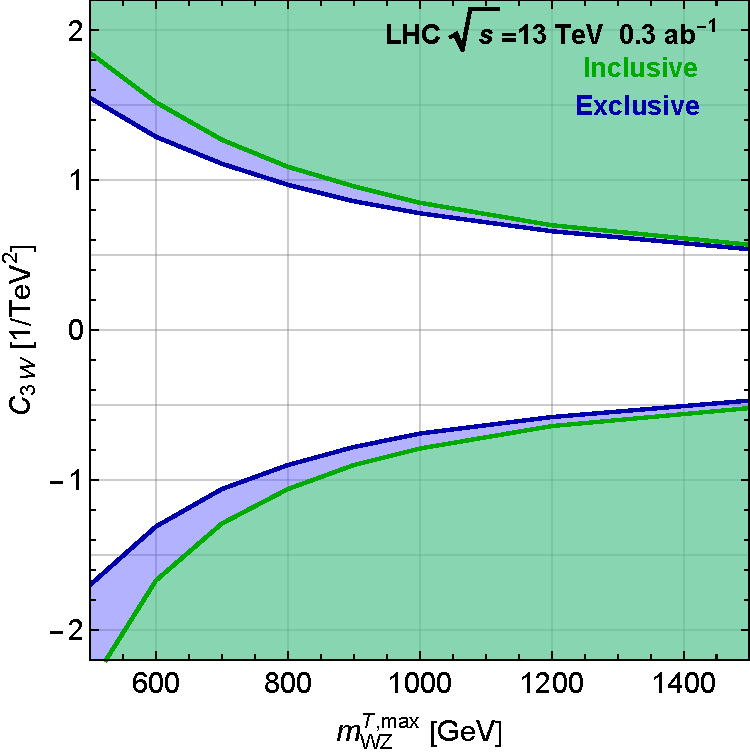
\includegraphics[width=0.39\textwidth]{\main/section4/LHC13_300.pdf}{}\hspace{2cm}
 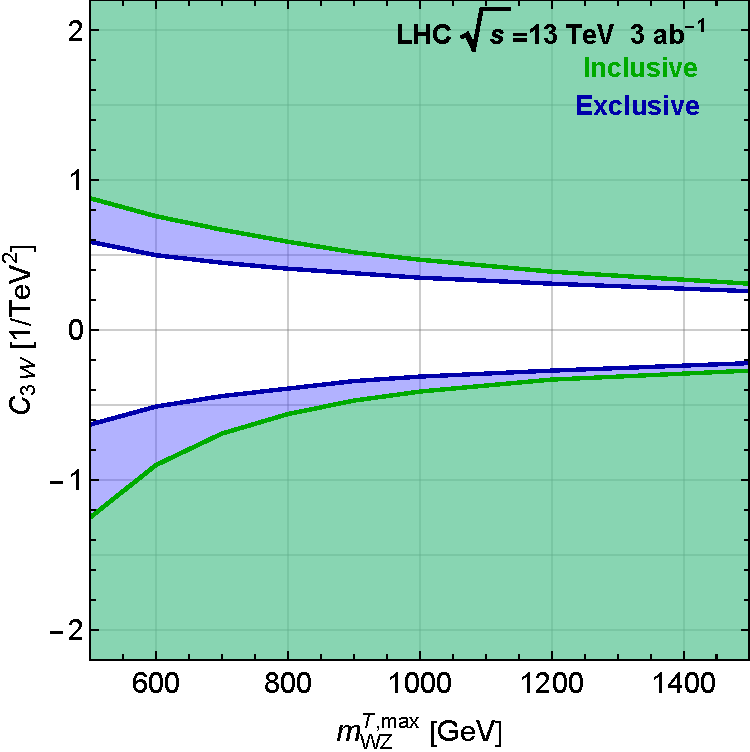
\includegraphics[width=0.39\textwidth]{\main/section4/LHC13_3000.pdf}{}
\end{center}
\caption{Bounds on the $C_{3W}$ Wilson coefficient for the inclusive and exclusive categories at the LHC 13 for 300 fb$^{-1}$ (left) and 3000 fb$^{-1}$ (right) of integrated luminosity.}
\label{fig:LHC13}
\end{figure}

\subsubsection*{HE-LHC}


We now estimate the reach of a future HE phase of the LHC with
$\sqrt{s}=27\;$TeV. For these preliminary results we adopt the same binning, both in $\phi_Z$ and in jet transverse momentum, of the previous section. We show the results in Fig.~\ref{fig:LHC27}. We found a slight increase of order $~30\%$ on the reach on $C_{3W}$. We expect that a dedicated HE analysis will lead to a further improvement of these bounds; this can be done by exploiting in a more efficient way the high energy tails of the differential distributions.  


  \begin{figure}[h!]
\begin{center}
 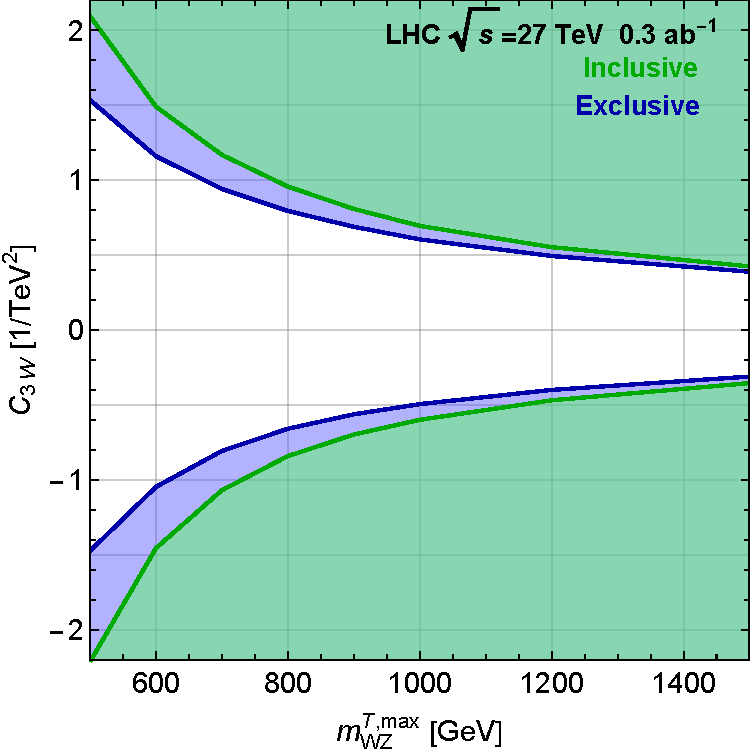
\includegraphics[width=0.39\textwidth]{\main/section4/LHC27_300.pdf}{}\hspace{2cm}
 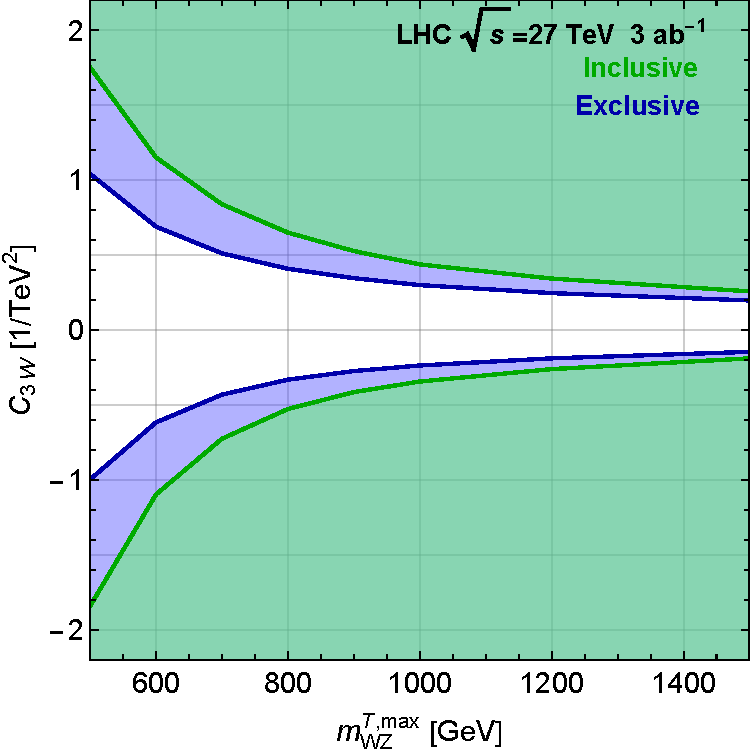
\includegraphics[width=0.39\textwidth]{\main/section4/LHC27_3000.pdf}{}
\end{center}
\caption{Bounds on the $C_{3W}$ Wilson coefficient for the inclusive and exclusive categories at the LHC 27 for 300 fb$^{-1}$ (left) and 3000 fb$^{-1}$ (right) of integrated luminosity.}
\label{fig:LHC27}
\end{figure}



%\subsection{VBF}
%\subsection{longitudinal VBS and di-Higgs} 
\subsubsection{Higgs pair production in vector-boson fusion at the HL-LHC}

\subfile{\main/section4/HHvbf}

\subsection{ Same-sign WW scattering at HL-LHC: a new strategy for the EFT-based analysis}
% 
\label{sect-ssWW}
\begin{center}
 {J. Kalinowski,$^{a} $
P. Koz{\'o}w,$^a$ S. Pokorski,$^a$
J. Rosiek,$^a$ M. Szleper$^b$ 
and
S. Tkaczyk$^c$\\
}
%\noindent
 {\small $^a$ Faculty of Physics, University of Warsaw, Warsaw,  Poland, \\
$^b$ National Center for Nuclear Research,  Warsaw, Poland, \\
$^c$  Fermi National Accelerator Laboratory, Batavia, IL 60510, USA.}
\end{center}
Although any statistically significant deviation in data from the  Standard Model(SM) predictions would be a manifestation of a BSM physics, the question is what we can learn about its scale and its strength before discovering new particles. The appropriate tool for answering this question is the Effective Field Theory(EFT) approach: the information about the  scale $\Lambda$ and the strength $C$ of new physics is encoded in  the Wilson coefficients of the higher dimension operators, $f_i=C^m/\Lambda^n$.
The usefulness of any EFT analysis of a given process relies on the assumption that only a few higher-dimension terms 
in the expansion ${\cal L}={\cal L}_{SM}+\sum_i f_i^{(6)}{\cal O}_i^{(6)}+ \sum_i f_i^{(8)}{\cal O}_i^{(6)}+\ldots$ 
provide adequate approximation to an unknown UV completion.   
This assumption  introduces a strong model-dependent aspect and therefore it is convenient to introduce the concept of EFT ``models" defined by the choice of operators  and the values of their Wilson coefficients $({\cal O}_i^{(d)},f_i^{(d)})$.  Our focus is on the proper use of the EFT "models" in their range of validity for the WW scattering in purely leptonic W decay channels where the $WW$ invariant mass cannot be determined experimentally  \cite{Kalinowski:2018oxd}.
%Strategies for future data analyses in case such a scenario indeed occurs are proposed.



Following a common practice we take one operator at a time setting others to 
zero,  which effectively defines the EFT ``model", 
and consider   the process 
$pp\rightarrow 2jW^+ W^+ \rightarrow 2j l^+\nu l'^+\nu^\prime$. 
The EFT ``model" can be maximally valid up to the invariant mass $M$ of the 
$W^+W^+$ system 
$M<\Lambda\leq M^U$, where $M^U=M^U(f)$ is the perturbative partial wave unitarity bound  in the chosen EFT "model".  
%In purely leptonic $W$ decay channel the invariant mass $M$ cannot be determined experimentally. 
If  the kinematic range $M_{max}$  at the LHC is greater than $\Lambda$, there is necessarily a 
contribution to observables from the region $\Lambda < M < M_{max}$.  
Two questions arise:1) what is the discovery region in the space $(\Lambda, f)$ for the chosen EFT "model", 2) if a deviation from  the SM predictions is indeed observed,
how to verify the chosen EFT  ``model"  by fitting it to a set of experimental distributions $D$ 
and in what range of $\Lambda, f_i$ such a fit is really meaningful?
%
%
\begin{figure}
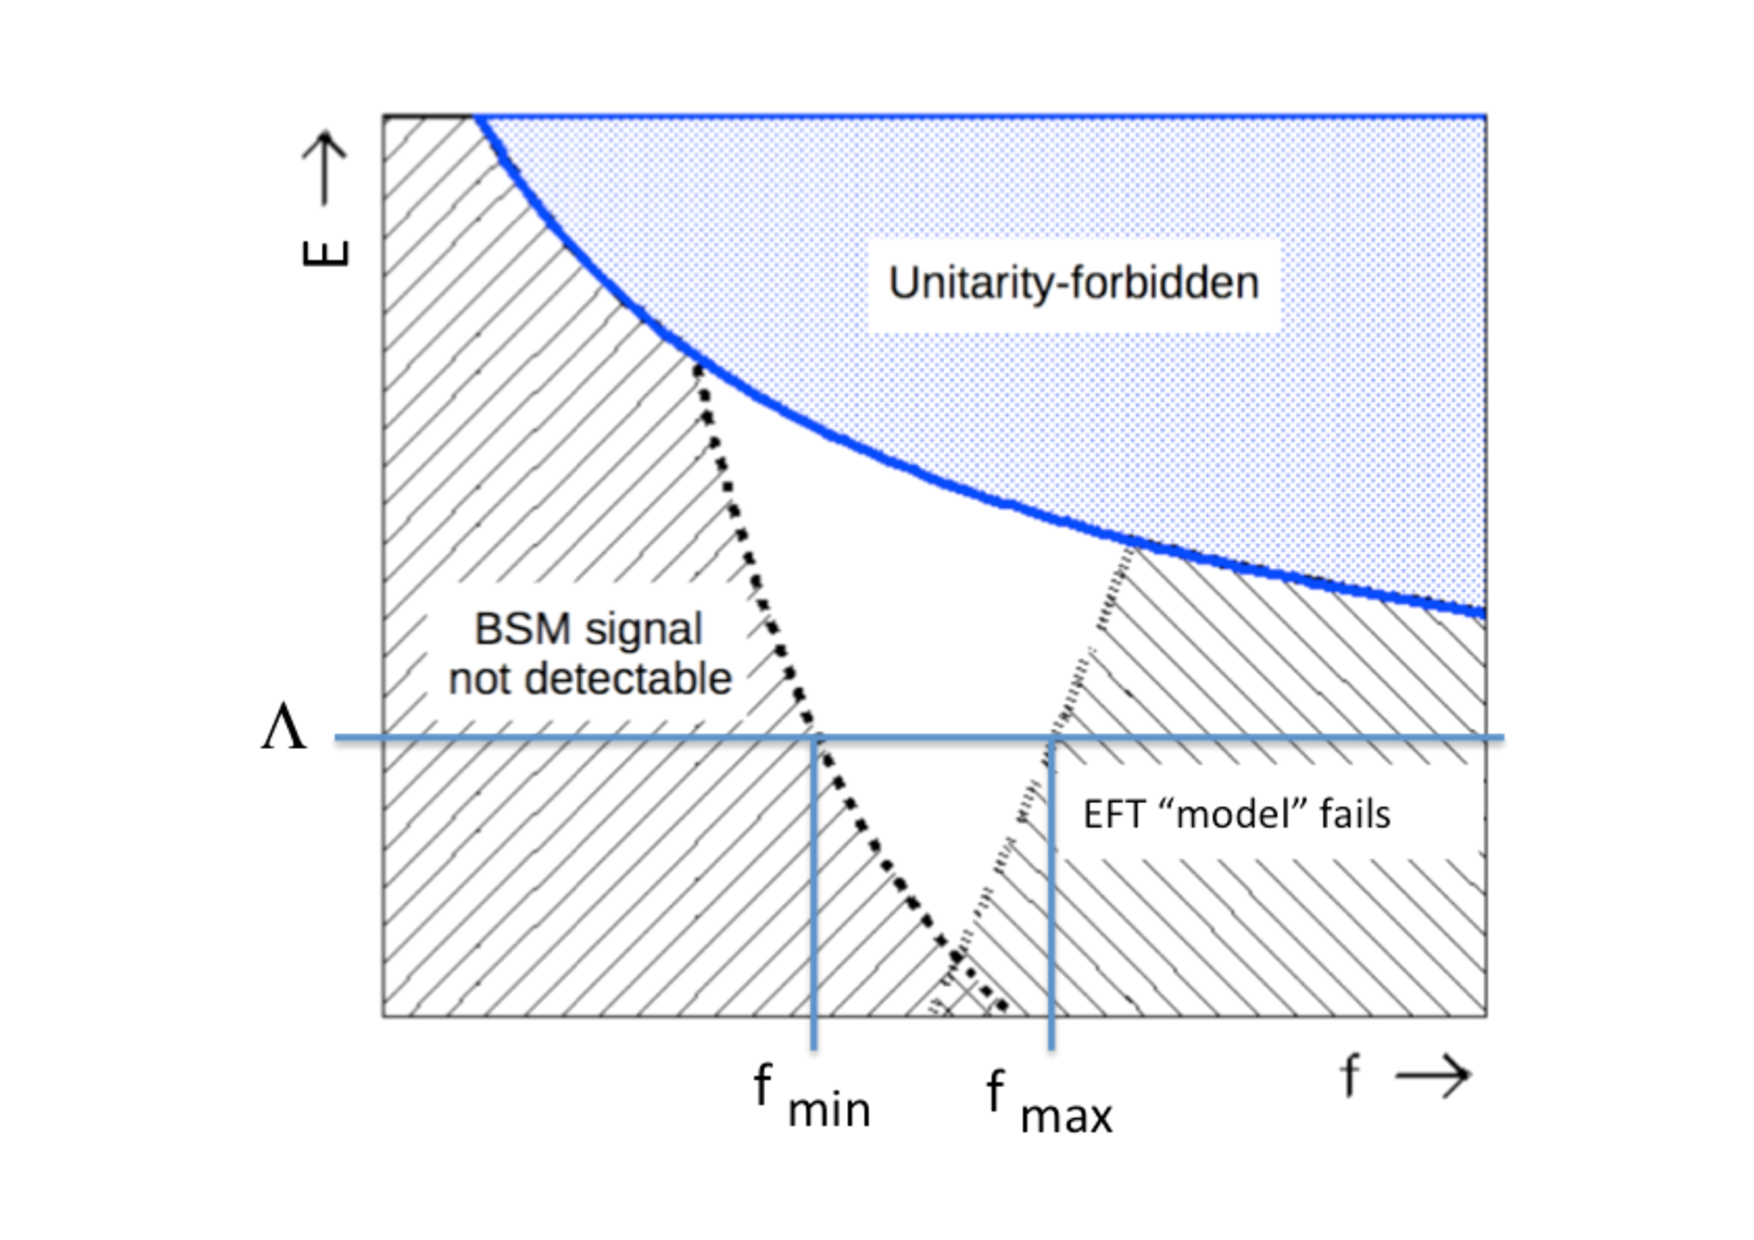
\includegraphics[width=0.8\linewidth]{\main/section4/cartoon3.pdf}
\caption{
Cartoon plot showing the regions in $f_i$ and $\Lambda$ in terms of BSM signal observability
and applicability of the EFT ``model"  for  the same-sign WW process with purely 
leptonic decays.  The white triangle shows the region
where the BSM physics can be studied within the chosen EFT "model".}
%\vspace{1cm}
\label{fig:cartoonplot}
\end{figure}
%

For a given EFT ``model" the unitarity bound is very different for  different helicity amplitudes.
As  $M^U$ we take  the $lowest$ value, universally for all helicity 
amplitudes. 
The BSM signal  $S$ of the EFT ``model" $({\cal O}_i^{(d)},\,f_i^{(d)})$ 
can be defined as the deviation of some observable $D$ from the SM prediction 
$S=D^{model}-D^{SM}$.
A quantitative estimate of the signal can be written as
\small
\begin{equation} 
D^{model}=\int^{\Lambda}_{2M_W}\frac{d\sigma}{dM} \Bigl|_{model} dM +\int_{\Lambda}^{M_{max}}\frac{d\sigma}{dM}\Bigr|_{SM} dM\,,
\label{dsigma}
\end{equation}
\normalsize
which comes uniquely from the operator that defines the ``model" in its range
of validity and assumes only the SM contribution in the region $M>\Lambda$.
BSM contribution from the region above $\Lambda$   may enhance the signal, but it may also 
preclude proper description of the data in the EFT  "model",
which makes sense {\it if and only if} this additional contribution is small enough  
compared to the contribution from the validity region.  
For a  quantitative estimate of this 
contribution we define a second estimate in which  all the helicity amplitudes above 
$\Lambda$ are assumed to remain 
constant at their respective values they reach at $\Lambda$
\small
\begin{equation}
D^{model}=\int^{\Lambda}_{2M_W}\frac{d\sigma}{dM}\Bigl|_{model} dM +\int_{\Lambda}^{M_{max}}\frac{d\sigma}{dM}\Bigr|_{A=const} dM.
\label{unitarized}
\end{equation}
\normalsize
For $\Lambda = \Lambda_{max}$ this prescription regularizes the helicity amplitudes that violate unitarity at $M^U$. 
We adopt the criterion that the EFT ``model" is tested for values of $(\Lambda\leq M^U, f_i)$ 
when the signals computed from Eq.(\ref{dsigma}) are statistically consistent 
within 2$\sigma$ with the signals computed with Eq.(\ref{unitarized}).

The observability of  the EFT "model" predictions imposes some minimum value of $f_{min}$, while the description within the EFT "model" imposes some 
maximum value of $f_{max}$ such that signal
estimates computed from Eqs.(\ref{dsigma}) and (\ref{unitarized}) remain 
statistically consistent.  
For $\Lambda=M^U$ a finite interval of $f_i$ values is possible, while 
for $\Lambda <M^U$ the  respective limits on $f_i$  depend on the actual value of $\Lambda$. It is illustrated in 
a cartoon plot in Fig.~\ref{fig:cartoonplot}, where the white "triangle" is bounded from 
above by the unitarity bound $M^U(f_i)$, from the left by the signal significance criterion 
and from the right by the consistency criterion.
The EFT "model" could be the right framework to describe the  BSM signal as long as the ``triangle"
shown in our cartoon plot is not empty.  






Our preferred strategy for data analysis is as follows:\\
a)  Measure  distributions $D$ that
offer the highest sensitivity to the studied EFT "model",\\
b) if deviations from the SM are observed, fit the values of 
$(\Lambda\leq M^U, f_i)$  according to 
Eq.(\ref{unitarized}),\\
c) using the fitted values of $f_i$ and $\Lambda$ recalculate 
$D$  templates 
according to 
Eq.(\ref{dsigma}),\\
d) check statistical consistency between estimates based on Eqs.(\ref{dsigma}) and (\ref{unitarized}). \\
 Physics conclusions from the obtained $(\Lambda, f_i)$ values can only be drawn
if such a consistency is found.  
%
%\begin{SCtable}[0.9][t]
%%\vspace{-2cm}
%\includegraphics[width=0.55\linewidth]{table.png}
%\caption{
%Estimated lower  and upper limits for BSM signal significance  for
%EFT consistency for each dimension-8 operator
%(positive and negative $f$ values), for the case when $\Lambda$ is equal
%to the unitarity bound,
%in the $W^+W^+$ scattering process at the LHC with 3 ab$^{-1}$.}
%%\vspace{1cm}
%\label{fig:cartoonplot}
%\end{SCtable}
%
Stability of the result against alternative 
regularization methods  would provide a measure of uncertainty of the procedure - too much
sensitivity to the region above $\Lambda$ means the procedure is destined to fail
and  that data cannot be described within the chosen EFT "model".

%
%{\bf 3. Results of simulations.}  

To demonstrate our strategy we considered EFT ``models" defined by 
one-at-a-time dimension-8 operator that affects $WWWW$ couplings. Details of the simulation of events for  the process 
$pp \to jj\mu^+\mu^+\nu\nu$ (at 14 TeV with 3/ab integrated luminosity) and their processing according to our strategy can be found in \cite{Kalinowski:2018oxd}. 
Assuming $\Lambda$ equal to the respective unitarity bounds,
the lower and upper limits for the values of $f$ for each dimension-8 operator, for positive
and negative $f$ values, as well as the applicability "triangles" in the $(\Lambda,f_i)$ plane for each operator have been caclulated.
  These limits define the (continuous) sets of testable 
EFT ``models" based on the choice of single dimension-8 operators. 
The "triangles"  turned to be rather narrow, but in most cases non-empty.

To summarize:  we  have introduced the concept of EFT ``models" defined by the choice of higher dimension operators and values of the Wilson coefficients and analyzed ``models" based on single dimension-8 operators at a time.  
We argue that usage of EFT ``models" in the analysis of purely
leptonic $W$ decay channels requires bounding the possible contribution from
the region $M_{WW} > \Lambda$, no longer described by the ``model",
and ensuring it does not significantly distort the measured distributions 
compared to what they would have looked from the region of EFT validity alone and 
propose a data analysis strategy to satisfy the above requirements.  We find that, with a possible exception of ${\cal O}_{S1}$, all dimension-8 operators which affect the
$WWWW$ quartic coupling have regions where
a 5$\sigma$ BSM signal can be observed at HL-LHC with 3 ab$^{-1}$ of data, while data
could be satisfactorily described using the EFT approach. 

%
%%%%%%%%%%%%%%%%%%%%%%%%%
Acknowledgments: 
%%%%%%%%%%%%%%%%%%%%%%%%%
Work partially supported by the National Science Centre (Poland) grants
DEC-2015/18/M/ST2/00054,  DEC-2016/23/G/ST2/04301 (SP), DEC-2015/19/B/ST2/02848 (JR) and 
HARMONIA project 
UMO-2015/18/M/ST2/00518  (JK). 
ST is supported by Fermi Research Alliance, LLC under Contract No.~De-AC02-07CH11359 with the US DoE.
%%%%%%%%%%%%%%%%%%%%%%%%%

\subsection{Testing the universal Higgs nonlinearity}
% 
\label{sect-illus}
\begin{center}
 {D. Liu,$^a$   I. Low,$^{a,b} $ Z. Yin, $^b$\\
}
%\noindent
 {\small $^a$ High Energy Physics Division, Argonne National Laboratory, Argonne, IL 60439, USA \\
$^b$ Department of Physics and Astronomy, Northwestern University, Evanston, IL 60208, USA.}
\end{center}
We initiate a phenomenological study of ``universal relations'' in composite Higgs models, which  are  dictated by nonlinear shift symmetries acting on the 125 GeV Higgs boson. These are relations among one Higgs couplings with two electroweak gauge bosons (HVV), two Higgses couplings with two electroweak gauge bosons (HHVV), one Higgs couplings with three electroweak gauge bosons (HVVV), as well as triple gauge boson couplings (TGC), which are all controlled by a single input parameter: the decay constant $f$ of the pseudo-Nambu-Goldstone Higgs boson.  Assuming custodial invariance in strong sector, the  relation is independent of the symmetry breaking pattern in the UV, for an arbitrary  symmetric coset $G/H$. The complete list of corrections to HVV, HHVV, HVVV and TGC couplings in composite Higgs models is presented to all orders in $1/f$, and up to four-derivative level,  without referring to a particular $G/H$. We then present several examples of  universal relations in ratios of coefficients which could be extracted experimentally. Measuring the universal relation requires a precision sensitive to effects of dimension-8 operators in the effective Lagrangian and highlights the importance of verifying the tensor structure of HHVV interactions in the standard model, which remains untested to date.


%%%%%%%%%%%%%%%%%%%%%%%%%
Acknowledgments: 
%%%%%%%%%%%%%%%%%%%%%%%%%
This work is supported in part by the U.S. Department of Energy under contracts No. DE-AC02-06CH11357 and No. DE-SC0010143.
%%%%%%%%%%%%%%%%%%%%%%%%%

\subsection{ Same-sign WW scattering: A comparison of the HL- and HE-LHC reach for the selected Dim8 operators within  the EFT approach}
% 
\label{sect-illus}
\begin{center}
 {G. Chaudhary,$^a$   J. Kalinowski,$^{b} $ M. Kaur, $^a$
P. Koz{\'o}w,$^b$ K. Sandeep,$^a$ M. Szleper$^c$ 
and
S. Tkaczyk$^d$\\
}
%\noindent
 {\small $^a$ University of Panjab, Chandigarh, India,\\
$^b$ Faculty of Physics, University of Warsaw, Warsaw,  Poland, \\
$^c$ National Center for Nuclear Research,  Warsaw, Poland, \\
$^d$  Fermi National Accelerator Laboratory, Batavia, IL 60510, USA.}
\end{center}

In Sect.\ref{sect-ssWW} a new strategy for the EFT-based analysis of the same-sign WW scattering  in the purely leptonic $W$ decay channels at the LHC has been proposed. Since in this process the scale of the WW scattering cannot be reconstructed experimentally, the main idea of the proposed strategy is to require that the dominant contribution to the observed signal should come from the EFT controlled region of the phase space. As a result, for the given EFT scale $\Lambda$ one expects a finite  interval of the Wilson coefficient,  from $f_{min}$ to $f_{max}$, where the BSM signal is observable and the EFT description can be trusted. Together with the unitarity bound  the $f_{min}$ and $f_{max}$ eventually will form a "trangle", as shown in the cartoon plot Fig.\ref{fig:cartoonplot}, where the BSM physics can be studied within the chosen EFT "model". 

Following the above strategy  we have compared the expected reach the expected reach for the dim-8 operator $O_{M6}$ at the HL- and HE-LHC  assuming the integrated luminosities 3/ab and ??/ab, respectively.  Fig.\ref{fig:fM6} shows the respective "triangles". 
\begin{figure}

\includegraphics[width=0.6\linewidth]{\main/section4/fM6.pdf}
\caption{
Regions in $f_{M6}$ and $\Lambda$ in terms of BSM signal observability
for the EFT ``model"  based on M6 operator at the HL- and HE-LHC.}
%\vspace{1cm}
\label{fig:fM6}
\end{figure}



%%%%%%%%%%%%%%%%%%%%%%%%%%%%%%%%%%%%%%%%%%%%%%%%%%%%%%%%%%%%%%%%%%%%%%%%%%%%%%%%%%%%%%%%%%%%%%%%%
%%%%%%%%%%%%%%%%%%%%%%%%%%%%%%%%%%%%%%%%%%%%%%%%%%%%%%%%%%%%%%%%%%%%%%%%%%%%%%%%%%%%%%%%%%%%%%%%%
%%%%%%%%%%%%%%%%%%%%%%%%%%%%%%%%%%%%%%%%%%%%%%%%%%%%%%%%%%%%%%%%%%%%%%%%%%%%%%%%%%%%%%%%%%%%%%%%%

\subsection{Dimension-6 EFT effects on Vector Boson Scattering at high energies}

\begin{center}
\bigskip\vspace{1cm}
{Roberto Covarelli$^{a}$ and  Raquel Gomez-Ambrosio$^{b}$}
\centerline{$^a${\it Univerist\'a di Torino and INFN sezione di Torino, Via Pietro Giuria 1, 10125, Turin, Italy}}
\centerline{$^b${\it Institute of Particle Physics Phenomenology, Durham University, Durham DH1 3LE, UK}}
\end{center}

%%%%%%%%%%%%%%%%%%%%%%%%%%%%%%%%%%
\noindent {\bf Introduction}\\
In this note we assess the sensitivity of vector boson scattering (VBS) processes to different dimension-6 ($\mathrm{dim=6}$) operators. We focus here on the $ZZ$ final state, decaying to 4 charged leptons. This experimental channel, currently statistically limited at the LHC \cite{Sirunyan:2017fvv}, will become more interesting at the HL-LHC because of the attainable selection purity. The full reconstruction of the final states also gives access to cleaner observables with respect to final states involving $W$ bosons, where neutrino 4-momenta must be inferred using approximated methods.
This analysis can nevertheless be repeated analogously to other VBS final states. 

In \cite{Gomez-Ambrosio:2018pnl} we studied the purely electroweak component of the $p p \to Z Z j j$ process, referred to as VBS(ZZ). Sensitivity to several $\mathrm{dim=6}$ operators has been demonstrated, as well as the impact of such EFT contribution on the VBS cross-section and triple and quartic gauge couplings (TGCs and QGCs). 

Here we update predictions for the HL-LHC setup and show the kinematic distributions for a handful of relevant operators. For the $\mathrm{dim=6}$ parametrisations we use the \emph{Warsaw basis} from \cite{Grzadkowski:2010es}, following the notation and classification from \cite{Jenkins:2013zja}. Other technical details can be found in the original publication \cite{Gomez-Ambrosio:2018pnl}.

\begin{figure}[h!]
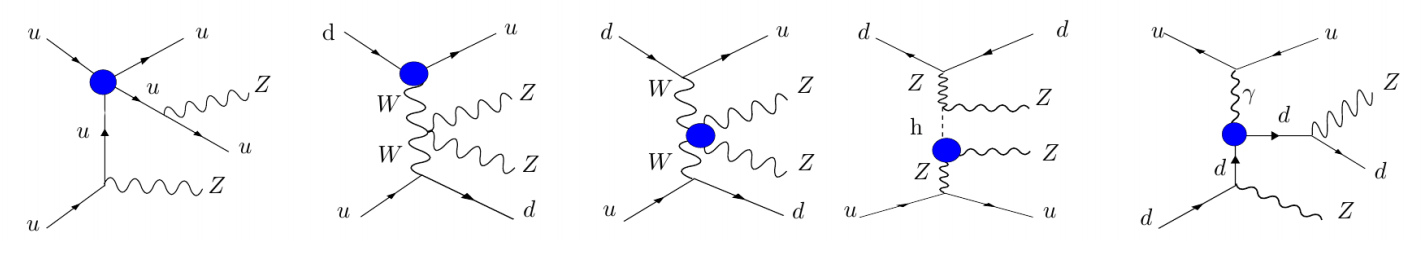
\includegraphics[scale=0.3]{\main/section4/feynmandiagramssignal.png}
\caption{Examples of some EFT diagrams for the VBS(ZZ) signal. The blobs represent $\mathrm{dim=6}$ insertions.}
\end{figure}

%{\large{\bf Effective Field Theory parametrization}} \\ \\
\noindent {\bf Effective Field Theory parametrization}\\
%
We consider a standard SMEFT parametrisation:

\begin{equation}
\mathcal{L}_{SMEFT} = \mathcal{L}_{SM} + \sum_i \frac{c_i}{\Lambda^2} \mathcal{O}_i^{(6)} + \dots 
\end{equation}
%
where the $\mathcal{O}^{(6)}_i$ represent a basis of $\mathrm{dim=6}$ operators built from SM fields and respecting the known gauge symmetries\footnote{In particular, we assume CP symmetry, neglecting the CP-odd operators since their impact on VBS cross-sections and differential distributions is negligible. However it is well known that certain variables of these processes (namely spin correlations and polarizations) can be sensible to CP-violation.}, and $c_i$ are the Wilson coefficients of the theory. Further, the SMEFT amplitudes and cross sections can be parametrised as
%
\begin{equation}
\mathcal{A}_{EFT} = \mathcal{A}_{SM} + \frac{g'}{\Lambda^2} \mathcal{A}_{6} +   \frac{g'^2}{\Lambda^4} \mathcal{A}_{8} + \dots 
\end{equation}
%
\begin{equation}
 \sigma_{EFT} \sim \vert \mathcal{A}_{SM} \vert^2 + {\color{red} 2\frac{g'}{\Lambda^2} \mathcal{A}_{SM} \mathcal{A}_{6} } + {\color{blue} \frac{g'2}{\Lambda^4} \left(  2 \mathcal{A}_{SM} \mathcal{A}_{8} + \vert \mathcal{A}_{6} \vert^2 \right)} + \dots
\end{equation}
%
Here, we assume the linear contribution (red) of the EFT effects to be leading. Analysis of the $\mathrm{dim=6}$ quadratic terms and the $\mathrm{dim=8}$ interference terms (both in blue) will be subject of further studies.  In particular, $\mathrm{dim=8}$ are commonly associated with quartic gauge couplings and such contribution, albeit subleading, would represent some added value to the linear $\mathrm{dim=6}$ prediction. \\
 
\noindent {\bf Definition of the fiducial region}\\
The VBS(ZZ) process has a very peculiar experimental signature, with two energetic forward jets and 4 identifiable charged leptons ($\ell, \ell' = \mu$ or $e$).
The electroweak component of the process $p p \to Z Z j j \to \ell \bar{\ell} \, \ell' \bar{\ell'} j j$ is defined and isolated through some experimental cuts. The ones used in the CMS analysis (in the measurement of the fiducial cross-section) can be found in \cite{Sirunyan:2017fvv}. Here we define a similarly VBS-enriched region, with a relaxed $m_{jj}$ selection: {\color{red} Editors, I'd like to have this in 2 columns but I don't want to mess up anything.... usepackage{multicol} didnt work unfortunately}
%

%\begin{multicols}{2}
\begin{itemize}
\item $p_T (j) > 30$ GeV
\item $\Delta \eta (j_1 j_2) > 2.4$
\item $ m_{jj} > 100$ GeV
\item \emph{on-shell} $Z_1,Z_2$ 
\end{itemize}
%\end{multicols}
%

%%%%%%%%%%%%%%%%%%%%%%%%%%%%%%%%%%%%%%%%%%%%%%%%%%%%%5
 
 
\noindent {\bf EFT analysis}\\ 
In tables~\ref{tab:signal} and \ref{tab:background} we show the sensitivities to different $\mathrm{dim=6}$ operators of the VBS(ZZ) process, as well as of its main background at LHC: the diboson production channel from quark-antiquark annihilation associated to gluon radiation (studied in depth by CMS for LHC runs I and II in \cite{Sirunyan:2018vkx}, QCD(ZZ)). 

Further, in figure \ref{fig:plots} we show differential distributions for a subset of the previous operators. In particular we chose the three operators that directly affect triple and quartic gauge couplings: {\color{red} this as well}

%\begin{multicols}{2}
\begin{itemize}
\item $\mathcal{O}_W = \epsilon^{ijk} W_{\mu}^{i \nu} W_{\nu}^{j \rho} W_{\rho}^{k \mu} $
\item $\mathcal{O}_{HW} = H^{\dagger} H W_{\mu \nu}^I W^{\mu \nu I}$
\item $\mathcal{O}_{HWB} = H^{\dagger} \tau^I H W_{\mu \nu}^I B^{\mu \nu}$
\end{itemize}
%\end{multicols}
 
However, as reported in tables~\ref{tab:signal} and \ref{tab:background}, there are other relevant operators for the VBS process, 
% in general and the TGC and QGC in particular. 
for example $\mathcal{O}_{\ell \ell}$, the 4-lepton operator that affects $G_F$, or $\mathcal{O}_{HB}$ that enters the $Z$ boson propagator. More details can be found for example in \cite{Ghezzi:2015vva}.
 
Figure \ref{fig:plots} should be interpreted as follows: we select one paradigmatic operator (for example $\mathcal{O}_W$), and see how much does its interference term affect the VBS and diboson signals ($2.5\%$ in this case). As the VBS(ZZ) cross section is still mostly unconstrained experimentally, while the QCD(ZZ) has a $21\%$ uncertainty in the 2-jet bin \cite{Sirunyan:2018vkx}, we know the bounds within which we can vary this coefficient. If we assume for example a $10 \%$ positive interference with the total cross-section, we observe that such a small contribution to the total cross-section can represent a large modification in certain bins of the differential distributions. This advantage is twofold: with this procedure we can select the optimal bin(s) for the study and fit of each EFT operator; and, by applying unitarity considerations, we can constrain the values of the Wilson coefficients further. In our example, a contribution of $10 \%$ in $\mathcal{O}_W$, still allowed for the total rate, has a large impact on the high energy bins of the $p_T (Z_1)$ distribution. 
\\
 
\noindent {\bf Conclusions}\\
The VBS(ZZ) and QCD(ZZ) final states, still largely unexplored at the LHC, will be an important source of constraints on $\mathrm{dim=6}$ EFT operators at the HL-LHC. We have shown the impact that values of Wilson coefficients still experimentally allowed have on differential distributions that are easily accessible experimentally in this channel. 

% 
\begin{figure}[htbp]
  \begin{minipage}[b]{0.5\textwidth}
    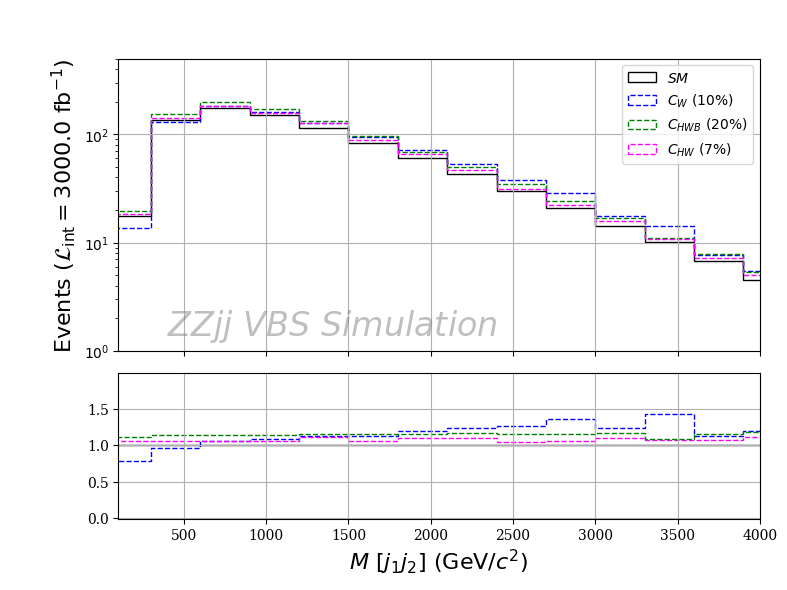
\includegraphics[width=1.02\textwidth]{\main/section4/mjj.png}
    %\caption{Picture 1}
    %\label{fig:1}
  \end{minipage}
  %
  \begin{minipage}[b]{0.5\textwidth}
    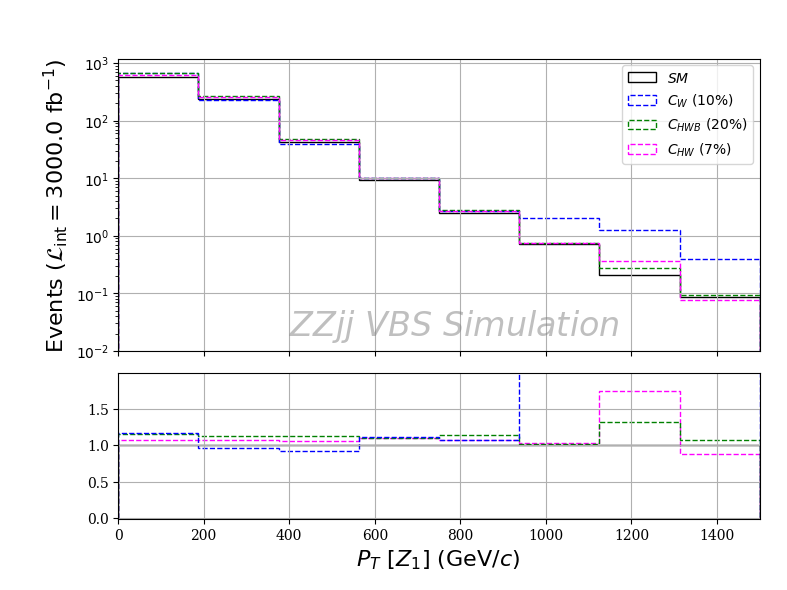
\includegraphics[width=1.02\textwidth]{\main/section4/ptz.png}
    %\caption{Picture 2}
    %\label{fig:2}
  \end{minipage}
  \caption{Two generic simulations showing the EFT effects on key differential distributions: invariant mass of the di-jet system (left) and transverse momentum of the leading Z boson (right). We selected arbitrary values for the Wilson coefficients $\lbrace c_W, c_{HW}, c_{HWB} \rbrace$}
  \label{fig:plots}
\end{figure}

%%%%%%%%%%%%%%%%%%%%%%%%%%%%%%%%%%%%%%%%%%%%%%%%%%%%%%%%%%%%%%%%%%

\begin{table*}[]
\begin{center}
\small
\begin{tabular}{|c|c|}%\hline
\hline
VBS Signal & Signal strengths (Linear EFT) \\
\hline
%\hline
 Class 1:  &  $\mathcal{O}_W = c_W \cdot 2.5 \%$ \\
 Class 3: & $\mathcal{O}_{HD} = c_{HD} \cdot 6.0 \%$ \\
 Class 4: & $ \mathcal{O}_{HW} = c_{HW} \cdot 5 \% $, $ \mathcal{O}_{CHB} = c_{HB} \cdot 0.2 \% $,  $ \mathcal{O}_{HWB} = c_{HWB} \cdot 14 \% $\\
 Class 7: & $ \mathcal{O}_{Hl^{(3)}} = c_{Hl^{(3)}} \cdot 48 \% $,
 $ \mathcal{O}_{Hq^{(1)}} = c_{Hq^{(1)}} \cdot 2 \% $, \\ 
 & $ \mathcal{O}_{Hq^{(3)}} = c_{Hq^{(3)}} \cdot 46 \% $,  $ \mathcal{O}_{Hu} = c_{Hu} \cdot 0.8 \% $ 
 \\
 Class 8a: $(L \bar{L})(L \bar{L})$  &  ($G_F \to$) $ \mathcal{O}_{\ell \ell} = c_{\ell \ell} \cdot 24 \% $ , 
 $ \mathcal{O}_{qq^{(1)}} = c_{qq^{(1)}} \cdot 12 \% $, \\ &
$ \mathcal{O}_{qq^{(11)}} = c_{qq^{(11)}} \cdot 14 \% $, 
$ \mathcal{O}_{qq^{(33)}} = c_{qq^{(33)}} \cdot 100 \% $, 
$ \mathcal{O}_{qq^{(31)}} = c_{qq^{(31)}} \cdot 75 \% $
 \\
\hline 
 \end{tabular}
  \caption{  Different sensitivities to each of the Warsaw basis operators. The operators that are not listed do not intervene in the process, or do it in a negligible way. Each sensitivity $\epsilon_i$ is calculated as $\epsilon_i  = \vert \frac{\sigma_{EFT} - \sigma_{SM}}{\sigma_{SM}} \vert$, and they include a standard EFT prefactor $\frac{v^2}{\Lambda^2}\vert_{\Lambda=1TeV}$ which needs to be taken into account if substituting values for the $c_i$ in the table. NB: we quote the absolute value for the sensitivities $\epsilon$.}
  \label{tab:signal}
\end{center}
\end{table*}


\begin{table*}[]
\begin{center}
\small
\begin{tabular}{|c|c|}%\hline
\hline
ZZ Diboson & Sensitivities (Linear EFT) \\
\hline
%\hline
 Class 1:  &  $\mathcal{O}_G = 2.5 \%$, \quad $\mathcal{O}_W = 2.5 \%$ \\
Class 3: & $\mathcal{O}_{HD} = 6.0 \%$ \\
Class 4: & $ \mathcal{O}_{CHW} = 0.2 \% $, $ \mathcal{O}_{CHG} =  8 \% $, $ \mathcal{O}_{CHB} =  0 \% $, $ \mathcal{O}_{CHWB} =  12 \% $ \\
Class 7: & $ \mathcal{O}_{Hl^{(3)}} = c_{Hl^{(3)}} \cdot 25 \% $ ,
$ \mathcal{O}_{Hq^{(1)}} = c_{Hq^{(1)}} \cdot 3 \% $, \\ & 
$ \mathcal{O}_{Hq^{(3)}} = c_{Hq^{(3)}} \cdot 31 \% $,
$ \mathcal{O}_{Hu} = c_{Hu} \cdot 1.1 \% $
%,$ \mathcal{O}_{Hu} = c_{Hd} \cdot 0.1 \% $
\\
Class 8a: $(L \bar{L})(L \bar{L})$  &  ($G_F \to$) $ \mathcal{O}_{\ell \ell} = c_{\ell \ell} \cdot 12 \% $ , $ \mathcal{O}_{qq^{(1)}} = c_{qq^{(1)}} \cdot 1.0 \% $, \\ &
$ \mathcal{O}_{qq^{(11)}} = c_{qq^{(11)}} \cdot 1.3 \% $, 
$ \mathcal{O}_{qq^{(33)}} = c_{qq^{(33)}} \cdot 8.4 \% $, 
$ \mathcal{O}_{qq^{(31)}} = c_{qq^{(31)}} \cdot 8.0 \% $
\\
\hline
 \end{tabular}
  \caption{Sensitivities to the different $\mathrm{dim=6}$ operators in the diboson production channel, main background for the VBS(ZZ) at LHC. A large sensitivity does not necessarily mean that a large EFT effect is expected, since the corresponding Wilson coefficient might as well be very small. %NB: we quote the absolute value for the sensitivities $\epsilon$.  
  }
  \label{tab:background}
\end{center}
\end{table*}
%%%%%%%%%%%%%%%%%%%%%%%%%%%%%%%%%%%%%%%%%%%%%%%%%%%%%%%%%%%%%%%%%%


 

%%%%%%%%%%%%%%%%%%%%%%%%%%%%%%%%%%%%%%%%%%%%%%%%%%%%%%%%%%%%%%%%%%%%%%%%%%%%%%%%%%%%%%%%%%%%%%%%%
%%%%%%%%%%%%%%%%%%%%%%%%%%%%%%%%%%%%%%%%%%%%%%%%%%%%%%%%%%%%%%%%%%%%%%%%%%%%%%%%%%%%%%%%%%%%%%%%%
%%%%%%%%%%%%%%%%%%%%%%%%%%%%%%%%%%%%%%%%%%%%%%%%%%%%%%%%%%%%%%%%%%%%%%%%%%%%%%%%%%%%%%%%%%%%%%%%%
%%%%%%%%%%%%%%%%%%%%%%%%%%%%%%%%%%%%%%%%%%%%%%%%%%%%%%%%%%%%%%%%%%%%%%%%%%%%%%%%%%%%%%%%%%%%%%%%%%

\clearpage

\end{document}
